\documentclass[12pt]{article}

\usepackage[utf8x]{inputenc}
\usepackage[L7x, T2A]{fontenc}
\usepackage[lithuanian]{babel}
\usepackage{vwcol}  
\usepackage{sectsty}
\usepackage{setspace}
\usepackage{fancyhdr}
\usepackage{graphicx}
\usepackage{ragged2e}
\usepackage{titlesec}
\usepackage{epsfig}
\usepackage{indentfirst}
\usepackage[top=2cm, bottom=2cm, left=3cm, right=1.5cm]{geometry}
\usepackage{makecell}
\usepackage[justification=centering]{caption}
\usepackage{titlesec}
\usepackage{fullpage}
\usepackage{amsmath,amssymb,amsthm,enumitem}
\usepackage{enumitem}
\usepackage{color}  
\usepackage[hypertexnames=false]{hyperref}
\hypersetup{
    colorlinks=true,
    linktoc=all,
    linkcolor={black},
    urlcolor={blue}
}
\usepackage[tocindentauto]{tocstyle}
\usetocstyle{standard}
\usepackage{eurosym}

\usepackage{svg}

\makeatletter
\expandafter\let\csname L7x-cmd\endcsname\@changed@cmd
\makeatother

\addto\extraspolish{\fontencoding{L7x}\selectfont}
\addto\noextraspolish{\fontencoding{\encodingdefault}\selectfont}

\setlength\parindent{1cm}

\title{VILNIAUS UNIVERSITETAS \\
MATEMATIKOS IR INFORMATIKOS FAKULTETAS \\
PROGRAMŲ SISTEMŲ KATEDRA}
\author{}
\date{}

\pagestyle{fancy}
\fancyhead{}
\fancyfoot{}
\fancyfoot[R]{\thepage}
\renewcommand{\headrulewidth}{0pt}
\renewcommand{\baselinestretch}{1.5}

\settocstylefeature[-1]{entryhook}{\Large\bfseries}

\begin{document}
	\clearpage
	\maketitle
	\thispagestyle{empty}

	\bigbreak
	\bigbreak
	\bigbreak
	\bigbreak

	\begin{center}
		\begin{Large}
			\textbf{Transporto priemonių skelbimų aplikacija} \\
		\end{Large}
		\begin{large}
			\textbf{Application for Vehicle Advertisement} \\
		\end{large}
		Programų sistemų inžinerijos I laboratorinis darbas \\

		\bigbreak
		\bigbreak
		\bigbreak
		\bigbreak
		\bigbreak
		\bigbreak
		\bigbreak
		\bigbreak
		\bigbreak

		\begin{tabular}{ll}
			Atliko:        & 2 kurso 5 grupės studentai \\
		               	   & Toma Burneikaitė \\
		               	   & Žygimantas Stongvilas \\
		                   & Mantas Jurčius \\
		                   & Rimvydas Meškauskas \\
			Darbo vadovas: & asist., dr. Vytautas Valaitis
		\end{tabular}

		\bigbreak
		\bigbreak
		\bigbreak
		\bigbreak
		\bigbreak
		\bigbreak
		\bigbreak
		\bigbreak
		\bigbreak

		Vilnius - 2018
	\end{center}
	\pagebreak
	
	\renewcommand{\baselinestretch}{0.5}
	\tableofcontents
	\renewcommand{\baselinestretch}{1.5}
	\pagebreak	
	
	\part*{Anotacija}
	\addcontentsline{toc}{part}{Anotacija}
	\begin{indent}
	Dokumentas parengtas kaip programų sistemos inžinerijos dalyko laboratorinis darbas, kuriame pateikiamas suprojektuotos sistemos aprašymas, reikalavimai bei dalykinės srities analizė. Programų sistemos architektūra apibrėžiama naudojantis 4+1 architektūros pjūvių modelį. Reikalavimai išskirstyti į funkcinius, nefunkcinius ir interfeiso reikalavimus. Dalykinės srities analizės metu atlikta išorinė bei vidinė proceso analizė įgyvendinamumo ir naudos analizė.
	\end{indent}
	\pagebreak
	
	\part*{Įvadas}
	\addcontentsline{toc}{part}{Įvadas}
	Šiame projektiniame darbe pristatomas transporto priemonių skelbimų programėlės „AutoINF“ įgyvendinimas. Mūsų vizija yra pasaulis, kuriame kiekvienas žmogus gali greitai, paprastai ir be vargo rasti reikiamą transporto priemonę, nesvarbu, kokiame Europos krašte ji bebūtų. Siekdami to mes užsibrėžiame tikslą sukurti mobiliesiems įrenginiams skirtą programėlę, kuri leistų pasiekti transporto priemonių skelbimus iš visos Europos. Idėja kilo todėl, kad dabar įvairių transporto priemonių skelbimai yra daugybėje skirtingų puslapių (šaltinių) ir norint susirasti naudingiausią pasiūlymą dažniausiai reikia pereiti per daugiau nei vieną puslapį. „AutoINF“ projekto tikslas yra sukurti programėlę, kuri supaprastintų transporto priemonių ieškojimo procesą ir padėtų vartotojui sutaupyti laiko tą darant, surinkdama visus skelbimus iš populiariausių Europos transporto priemonių skelbimų puslapių pagal vartotojo nurodytus kriterijus. Taip pat norima, kad programėle būtų paprasta naudotis ir kad ši programėlė sugebėtų pateikti kuo daugiau vartotojui aktualios informacijos apie tai, ko jis ieško.
	\pagebreak
	
	\part*{Projektavimas}
	\addcontentsline{toc}{part}{Projektavimas}

	Šioje dalyje aprašoma sistemos architektūra naudojant 4+1 architektūros pjūvių modėlį.
	
	\section{Užduotys ir jų vykdymo scenarijai}
	Šiame skyriuje pavaizduotos ir aprašytos sistemos vartotojų užduotys bei jų vykdymo scenarijai.
	\subsection{Sistemos vykdomos užduotys}
	Žemiau esančiame \ref{UseCase} paveikslėlyje pavaizduoti tikslai, kurių siekia sistema besinaudojantys agentai - automobilių ieškantys vartotojai bei sistemos administratoriai. Į sistemą žiūrima kaip į vieną visumą, neatskleidžiant jos implementacijos detalių.
	
	\begin{figure}[h]
		\begin{center}
			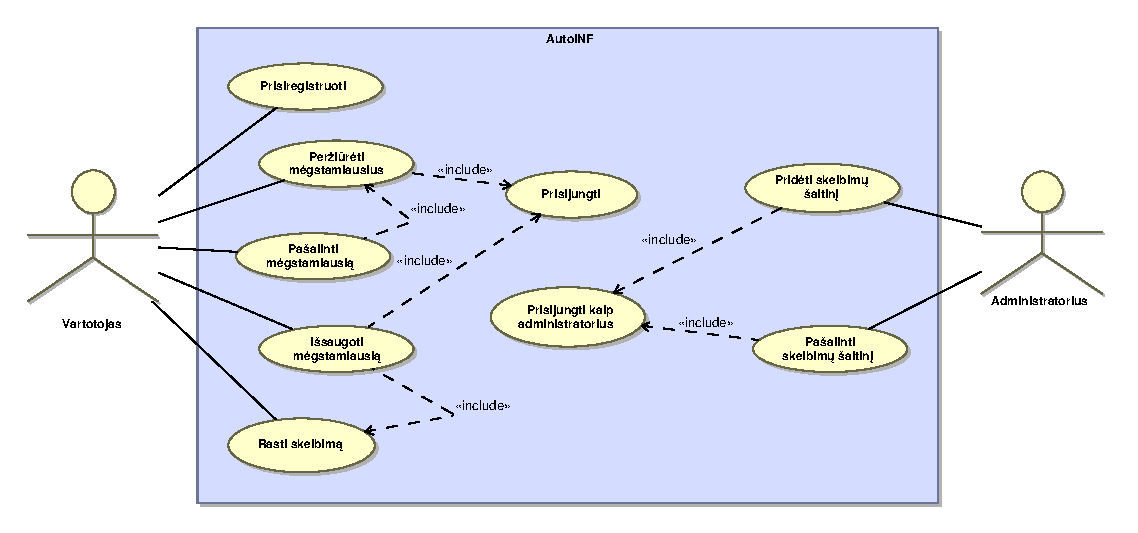
\includegraphics[width=\textwidth]{Tikslai.eps}
			\caption{Sistemos užduočių diagrama\label{UseCase}}
		\end{center}
	\end{figure}
	
	%\ref{UseCase} paveikslėlyje yra pavaizduoti tikslai, kurių siekia sistema besinaudojantys agentai - vartotojas ir administratorius
	\pagebreak

	\ref{UseCaseUser} paveikslėlyje pateiktos vartotojui prieinamos „AutoINF“ funkcijos: registracija, prisijungimas, peržiūrėti mėgstamiausius, pašalinti mėgstamiausią, išsaugoti mėgstamiausią, rasti skelbimą. Daugiau informacijos apie šias funkcijas yra tolimesnėse (\ref{RegisterSeq} - \ref{ViewFavSeq} pav.) sekų diagramose.
	
	\begin{figure}[h]
		\begin{center}
			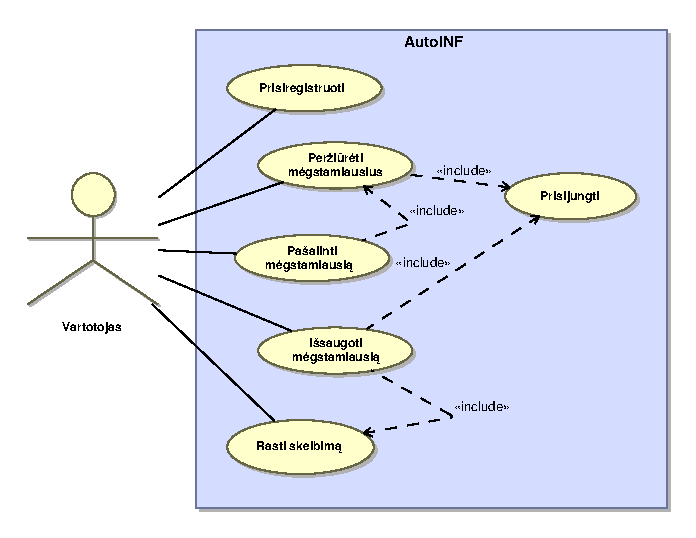
\includegraphics[width=0.7\textwidth]{TikslaiVartotojas.eps}
			\caption{Sistemos užduočių diagrama iš vartotojo perspektyvos\label{UseCaseUser}}
		\end{center}
	\end{figure}
	
%	\ref{UseCaseUser} paveikslėlyje pateiktos vartotojui prieinamos „AutoINF“ funkcijos: registracija, prisijungimas, peržiūrėti mėgstamiausius, pašalinti mėgstamiausius, išsaugoti mėgstamiausius, rasti skelbimą. Plačiau apie šias funkcijas rašoma tolimesnėse sekų diagramose.
	\pagebreak	
	
	\ref{UseCaseAdmin} paveikslėlyje pateiktos administratoriui prieinamos „AutoINF“ funkcijos: pridėti skelbimų šaltinį, pašalinti skelbimų šaltinį, pašalinti vartotojo paskyrą. Šios funkcijos labiau išplėtojamos tolimesnėje (\ref{ManSouSeq} pav.) sekų diagramoje. Administratorius prisijungia taip pat, kaip ir vartotojas, tik jam suteiktos administratoriaus teisės.	
	
	\begin{figure}[h]
		\begin{center}
			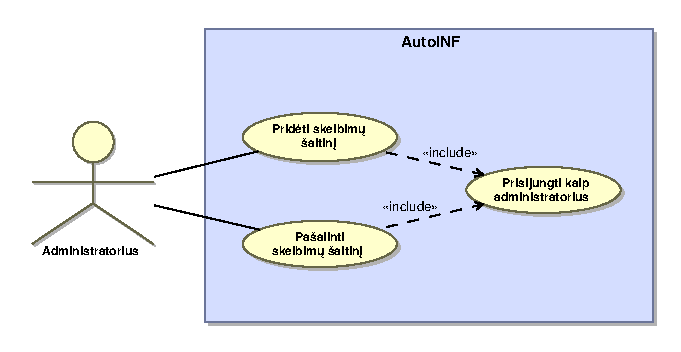
\includegraphics[width=0.7\textwidth]{TikslaiAdministratorius.eps}
			\caption{Sistemos užduočių diagrama iš administratoriaus perspektyvos\label{UseCaseAdmin}}
		\end{center}
	\end{figure}	
	
	\pagebreak
	
	\subsection{Užduoties „Prisiregistruoti“ įgyvendinimas}
	
	Vartotojo registracijos sistemoje užduoties vykdymas pavaizduotas \ref{RegisterSeq} paveikslėlyje. Vartotojas, atidaręs registracijos langą, turi suvesti prisiregistravimo duomenis. Paspaudus registracijos mygtuką, aplikacija patikrina, ar duomenys suvesti reikiamu formatu. Jei formatas teisingas, tai duomenys išsaugomi duomenų bazėje. Tada vartotojas yra infomuojamas apie sėkmingą registraciją ir yra prijungiamas prie sistemos.	
	
	\begin{figure}[h]
		\begin{center}
			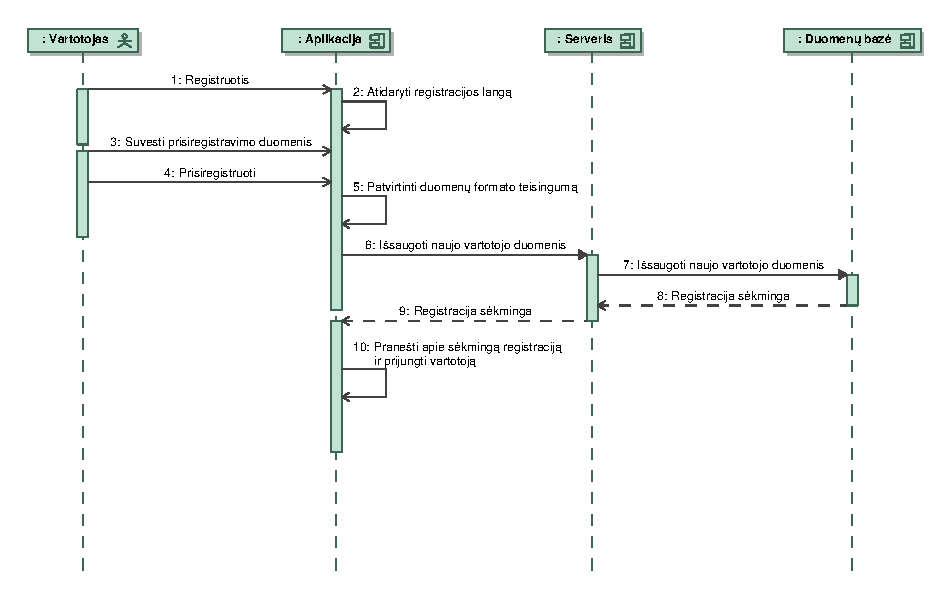
\includegraphics[width=\textwidth]{Prisiregistruoti.eps}
			\caption{Užduoties „Prisiregistruoti“ sekų diagrama\label{RegisterSeq}}
		\end{center}
	\end{figure}
	
	\pagebreak
	
	\subsection{Užduoties „Prisijungti“ įgyvendinimas}
	Vartotojo prisijungimo sistemoje užduoties vykdymas pavaizduotas \ref{LogInSeq} paveikslėlyje. Vartotojas, atidaręs prisijungimo langą, turi suvesti prisijungimo duomenis ir tada paspaudus prisijungimo mygtuką, duomenų bazėje yra patikrinama, ar toks vartotojas egzistuoja. Vartotojui prisijungus atsidaro pagrindinis langas, kuriame atsiranda funkcijos, prieinamos tik registruotiems vartotojams.
	\begin{figure}[h]
		\begin{center}
			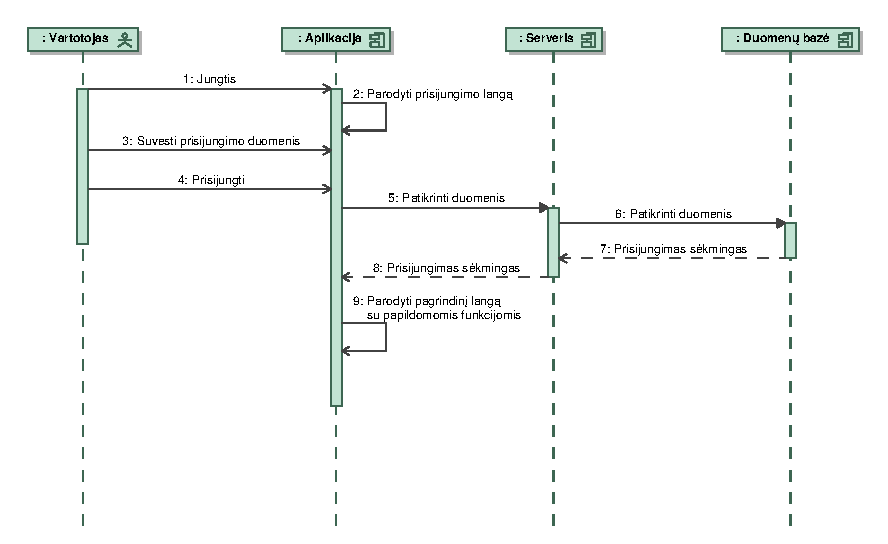
\includegraphics[width=\textwidth]{Prisijungti.eps}
			\caption{Užduoties „Prisijungti“ sekų diagrama\label{LogInSeq}}
		\end{center}
	\end{figure}
	

	\pagebreak
	
	\subsection{Užduoties „Rasti skelbimą“ įgyvendinimas}
	Skelbimų ieškojimo sistemoje užduoties vykdymas pavaizduotas \ref{FindAdvertSeq} paveikslėlyje. Vartotojas nebūtinai turi būti prisijungęs, kad galėtų pasinaudoti šia sistemos funkcija. Pirmiausia vartotojas turi pagrindiniame lange įvesti paieškos kriterijus (kai kurie filtrai yra privalomi). Paspaudus paieškos mygtuką, sistema suranda filtrą atitinkančius skelbimus ir juos parodo. Vartotojui paspaudus ant skelbimo atsidaro skelbimo langas.
	\begin{figure}[h]
		\begin{center}
			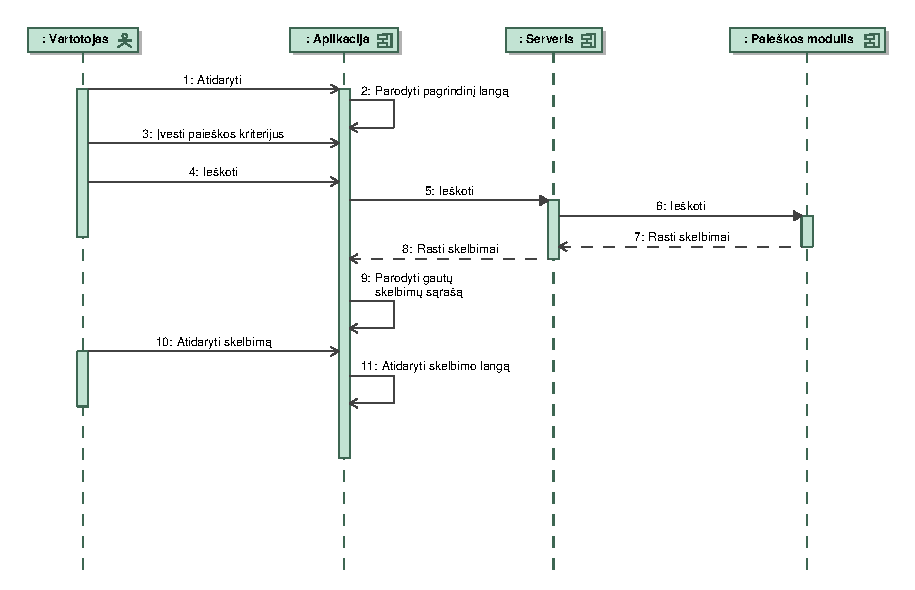
\includegraphics[width=\textwidth]{RastiSkelbima.eps}
			\caption{Užduoties „Rasti skelbimą“ sekų diagrama\label{FindAdvertSeq}}
		\end{center}
	\end{figure}
	
	
	\pagebreak
	
	\subsection{Užduoties „Išsaugoti mėgstamiausią“ įgyvendinimas}
	Mėgstamo skelbimo išsaugojimo užduoties vykdymas pavaizduotas \ref{SaveFavSeq} paveikslėlyje. Ši funkcija yra pasiekiama tada ir tik tada, kai vartotojas yra prisijungęs prie sistemos. Norėdamas išsaugoti skelbimą, vartotojas pirmiausia turi susirasti skelbimą ir tada  paspausti šio skelbimo išsaugojimo mygtuką. Apie sėkmingą skelbimo išsaugojimą vartotojas yra informuojamas.
	\begin{figure}[h]
		\begin{center}
			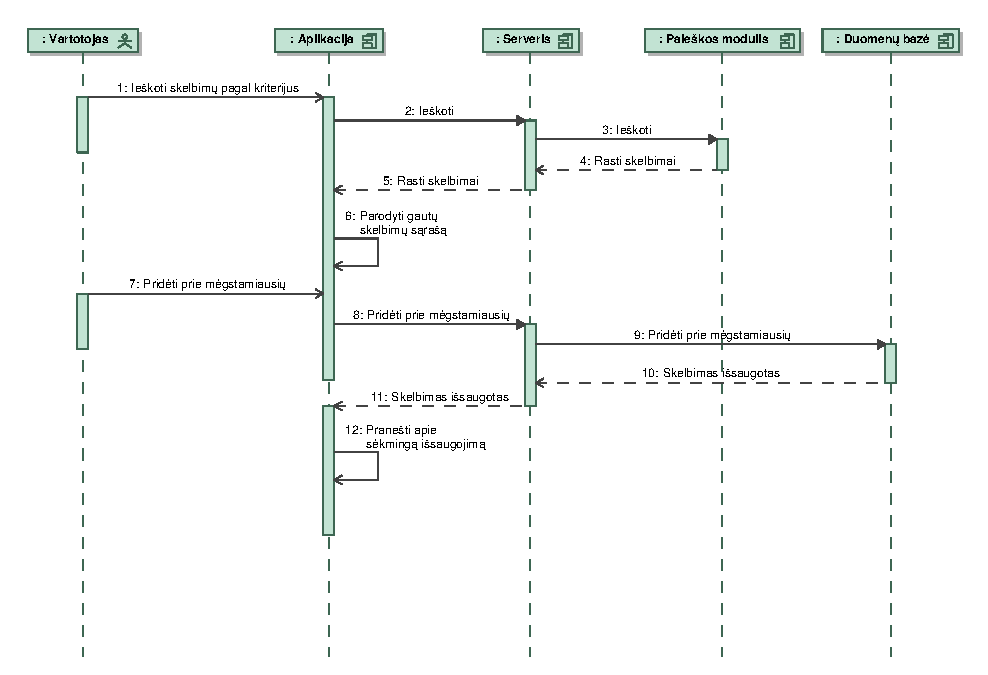
\includegraphics[width=\textwidth]{IssaugotiMegstamiausia.eps}
			\caption{Užduoties „Išsaugoti mėgstamiausią“ sekų diagrama\label{SaveFavSeq}}
		\end{center}
	\end{figure}
	
	
	\pagebreak
	
	\subsection{Užduoties „Pašalinti mėgstamiausią“ įgyvendinimas}
	Mėgstamo skelbimo pašalinimo užduoties vykdymas  pavaizduotas \ref{DelFavSeq} paveikslėlyje. Ši funkcija yra pasiekiama tada ir tik tada, kai vartotojas yra prisijungęs prie sistemos bei yra išsaugojęs bent vieną mėgstamą skelbimą. Pirmiausia vartotojas atsidaro mėgstamiausių skelbimų sąrašą. Tada pasirenka, kurį skelbimą jis nori pašalinti, ir paspaudžia pašalinimo mygtuką. Sėkmingai pašalinus skelbimą iš sąrašo, šis sąrašas yra atnaujinamas.
	\begin{figure}[h]
		\begin{center}
			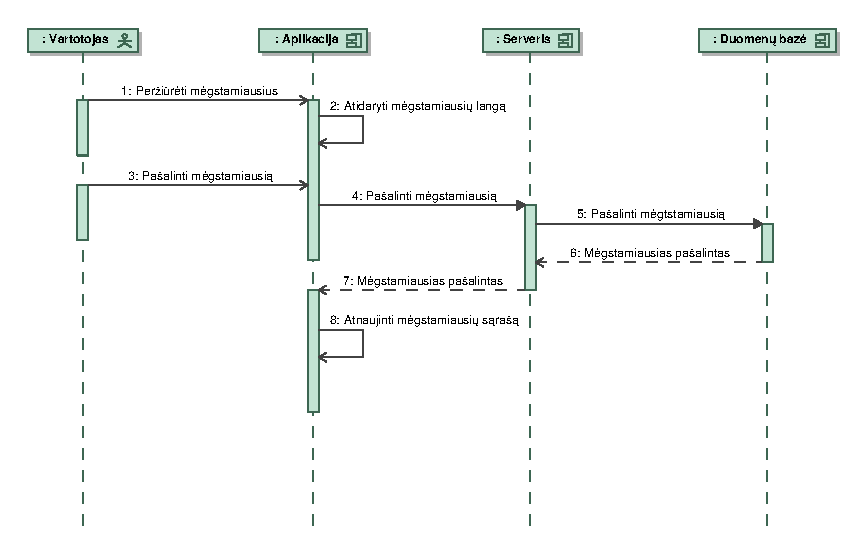
\includegraphics[width=\textwidth]{PasalintiMegstamiausia.eps}
			\caption{Užduoties „Pašalinti mėgstamiausią“ sekų diagrama\label{DelFavSeq}}
		\end{center}
	\end{figure}
	
	\pagebreak
	
	\subsection{Užduoties „Peržiūrėti mėgstamiausius“ įgyvendinimas}
	Mėgstamiausių skelbimų peržiūrėjimo užduoties vykdymas pavaizduotas \ref{ViewFavSeq} paveikslėlyje. Ši funkcijas pasiekiama tada ir tik tada, kai vartotojas yra prisijungęs prie sistemos. Vartotojui pasirinkus mėgstamiausių skelbimų langą, sistema parodo šio vartotojo mėgstamiausių skelbimų sarašą.
	\begin{figure}[h]
		\begin{center}
			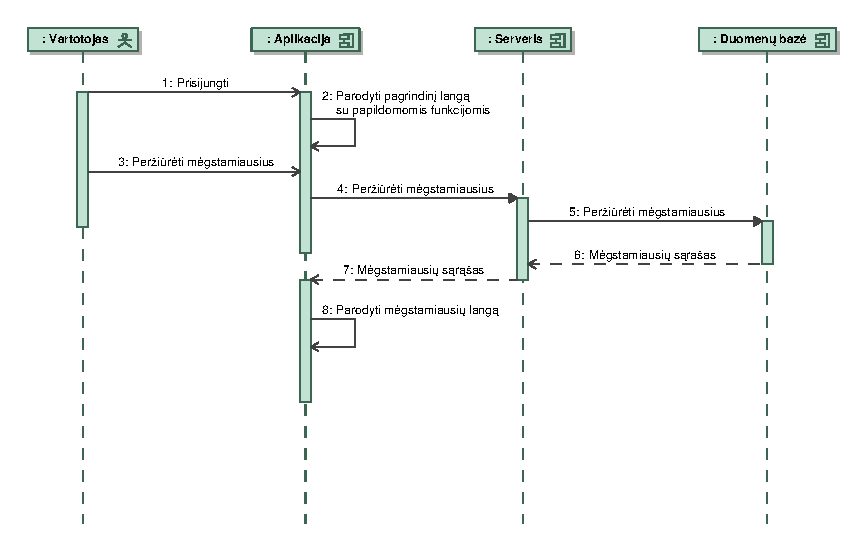
\includegraphics[width=\textwidth]{PerziuretiMegstamiausius.eps}
			\caption{Užduoties „Peržiūrėti mėgstamiausius“ sekų diagrama\label{ViewFavSeq}}
		\end{center}
	\end{figure}
	
	\pagebreak
	
	\subsection{Užduoties „Tvarkyti skelbimų šaltinius“ įgyvendinimas}
	Skelbimų šaltinių tvarkymo užduoties vykdymas yra pavaizduotas \ref{ManSouSeq} paveikslėlyje. Šia funkcija gali pasinaudoti tik administratorius. Administratorius, atsidaręs skalbimų šaltinių langą, gali pasirinkti, ką jis nori su šaltiniais daryti: pridėti naują skelbimų šaltinį ar pašalinti jau pridėtą šaltinį. Norėdamas pridėti šaltinį, administratorius spaudžia mygtuką, skirtą naujam šaltiniui pridėti, o siekdamas pašalinti skelbimą, administratorius turi pasirinkti šaltinį iš šaltinių sąrašo ir pasirinkti šaltinio pašalinimą. Tiek po šaltinio pridėjimo, tiek po šaltinio pašalinimo skelbimų šaltinių sąrašas yra atnaujinamas.
	\begin{figure}[h]
		\begin{center}
			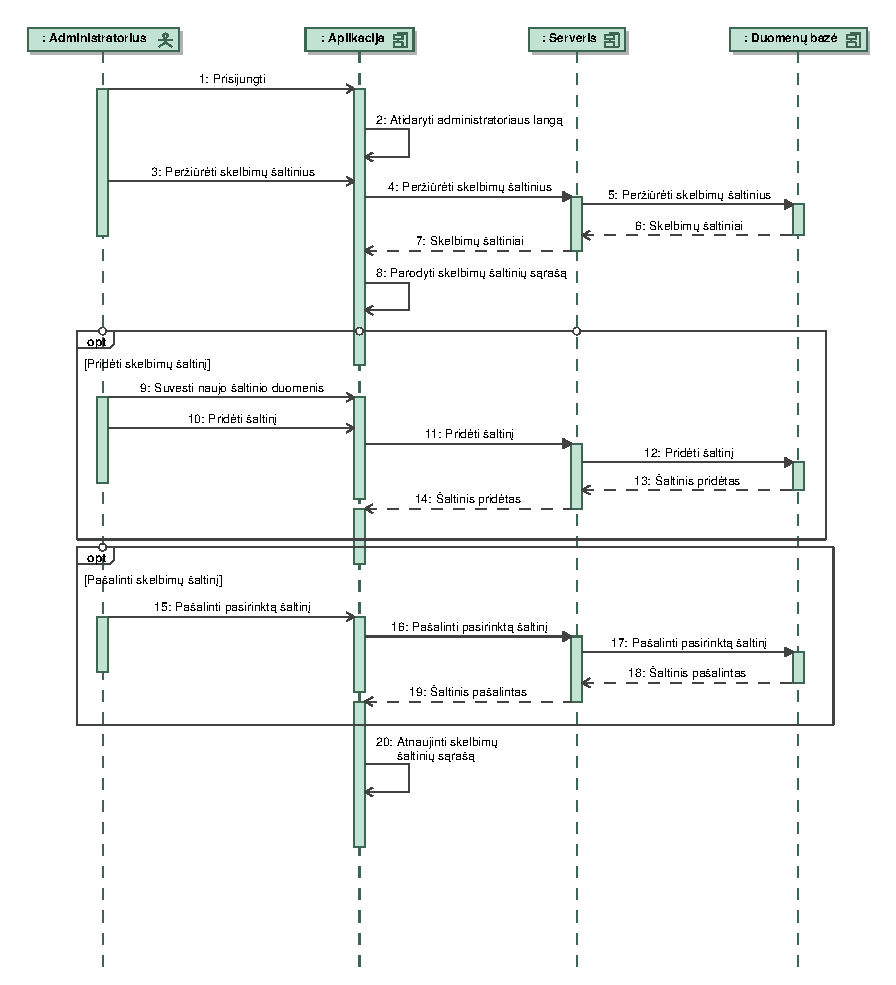
\includegraphics[width=0.75\textwidth]{TvarkytiSkelbimuSaltinius.eps}
			\caption{Užduoties „Tvarkyti skelbimų šaltinius“ sekų diagrama\label{ManSouSeq}}
		\end{center}
	\end{figure}

	\pagebreak
	
	\section{Struktūrinis programų sistemos modelis}
	Šiame skyriuje yra pateikta sistemos klasių diagrama ir, pasitelkiant objektų diagramą, parodytas sistemos naudojimo pavyzdys.
	\subsection{Klasių diagrama}
	
	Žemiau pateiktame \ref{ClassDiagram} paveikslėlyje yra išskirtos pagrindinės esybės, kurios yra naudojamos sistemoje. Klases siejantys ryšiai pasižymi kardinalumu. Kitaip sakant, nustatytas konkretus ryšių skaičius ar skaičių aibė, kurios turės klasės egzempliorius su tam tikros kitos klasės egzemplioriais.
	
	\begin{figure}[h]
		\begin{center}
			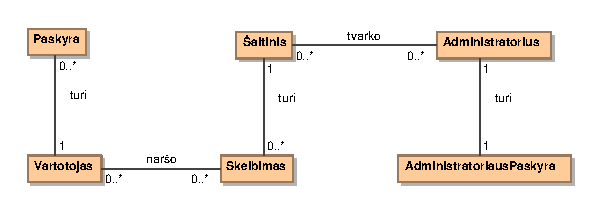
\includegraphics[width=0.9\textwidth]{KlasiuDiagrama.eps}
			\caption{Klasių diagrama\label{ClassDiagram}}
		\end{center}
	\end{figure}
	
	Šioje sistemoje egzistuoja dviejų rūšių paskyros: paprasta paskyra ir administratoriaus paskyra. Paprastas vartotojas gali turėti daug paskyrų (pvz.: pamiršta visus duomenis apie savo paskyrą, tai jis gali susikurti naują), o viena paskyra priklauso tik vienam vartotojui. Administratorius gali turėti tik vieną paskyrą: vartotojui, kuriam suteikiamos administratoriaus teisės, išduodamas vienkartinis kodas, kurį įvedus sukuriama speciali administratoriaus paskyra. Administratorius tvarko šaltinius (t.y. prideda arba pašalina šaltinius). Kiekvienas šaltinis gali būti tvarkomas kelių arministratorių ir taip pat kiekvienas administratorius gali tvarkyti kelis šaltinius. Vartotojai gali naršyti daug skelbimų ir visi kelbimai gali būti naršomi kelių vartotojų. Visi skelbimai yra paimti iš kokių nors šaltinių. Kiekvienas skelbimas gali būti paimtas tik iš vieno šaltinio, tačiau kiekvienas šaltiniai gali turėti daug skelbimų.
	\pagebreak
	
	\subsection{Objektų diagrama}
	
	Šiame skyrelyje esančios objektų diagramos iš esmės patvirtina anksčiau pateiktą klasių diagramą. Taip pat pateikia tipinį pavyzdžį, kaip klasės bus naudojamos sistemoje.
	
	\begin{figure}[h]
		\begin{center}
			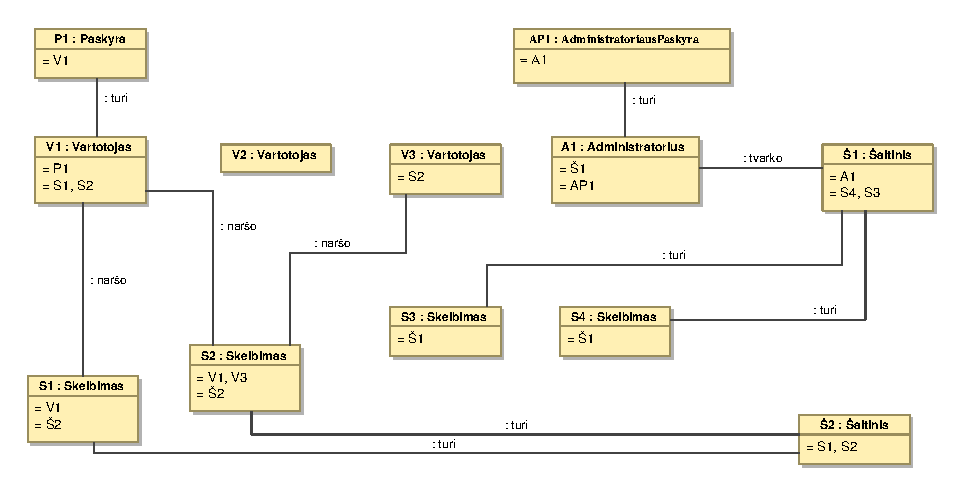
\includegraphics[width=\textwidth]{ObjektuDiagrama.eps}
			\caption{Objektų diagrama\label{ObjectDiagram}}
		\end{center}
	\end{figure}
	
	Aukščiau esančiame \ref{ObjectDiagram} paveikslėlyje parodyta tipinė sistemos situacija, kai yra sukurtos dvi paskyros: viena yra vartotojo, kita - administratoriaus. Taip pat yra dar du vartotojai, iš kurių vienas tuo momentu nieko nedaro sistemoje, kol kitas kartu su registruotu vartotoju naršo skelbimus (keli vartotojai gali naršyti tą patį skelbimą vienu metu). Taip pat yra keturi skelbimai, ir visi priklauso kažkuriam vienam šaltiniui, kol šaltiniai turi daugiau nei po vieną skelbimą (šaltiniai gali ir neturėti skelbimų). Taip pat iš diagramos galima matyti, kad administratorius gali tvarkyti šaltinius.
	\pagebreak
	
	\section{Programų sistemos komponentai}
	
	Šiame skyriuje yra pavaizduoti sistemos komponentai. Sistemos komponentų dekompozicija įgyvendinta „top-down“ būdu.	
	
	\subsection{Konteksto diagrama}
	Abstrakčiausias (aukščiausias) komponentų struktūros lygis parodomas \ref{Components1} paveikslėlyje.
	\begin{figure}[h]
		\begin{center}
			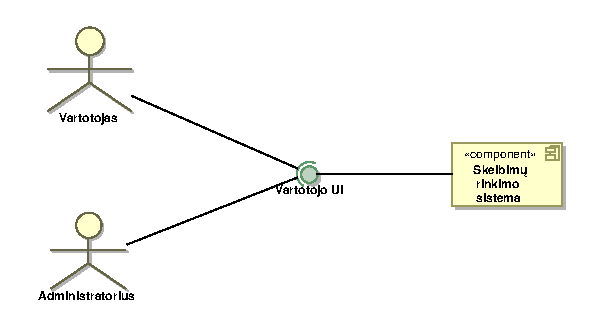
\includegraphics[width=0.9\textwidth]{Komponentai1.eps}
			\caption{Konteksto komponentų diagrama\label{Components1}}
		\end{center}
	\end{figure}
	
	 Visa sistema laikoma kaip vienas darinys ir parodoma sąsaja su išore:
	
	\begin{itemize}	
		\item Interfeisai, kuriais išoriniai vartotojai naudojasi visa sistema
		\item Išorinių sistemų interfesiai, kuriais naudojasi sistema
	\end{itemize}
	
	Tiek vartotojas, tiek administratorius turi naudotis tuo pačiu vartotojo UI interfeisu. To priežastis yra ta, kad abu vartotojai naudojasi ta pačia sistema, tik su šiek tiek skirtingomis galimybėmis.	
	\pagebreak

	\subsection{Skelbimų rinkimo sistemos dekompozicija}
	Žemiau esančiame \ref{Components2} paveikslėlyje detalizuojamas \ref{Components1} paveikslėlyje esantis „Skelbimų rinkimo sistema“ komponentas.
	\begin{figure}[h]
		\begin{center}
			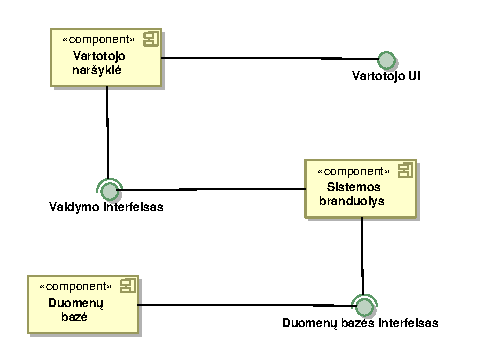
\includegraphics[width=0.9\textwidth]{Komponentai2.eps}
			\caption{Skelbimų rinkimo sistemos komponento dekompozicija\label{Components2}}
		\end{center}
	\end{figure}

	\textbf{Vartotojo naršyklė} - komponentas, sukuriantis vartotojo interfeisą bei vykdantis komuni-kaciją tarp vartotojo ir sistemos branduolio.

	
	\textbf{Sistemos branduolys} - komponentas, priimantis prašymus iš vartotojo naršyklės, kontroliuojantis duomenų gavimą ar išsaugojimą duomenų bazėje bei siunčiantis duomenis vartotojo naršyklei.

	
	\textbf{Duomenų bazė} - komponentas, kuriame saugoma informacija apie registruotus vartotojus ir kartu tos paskyros mėgstamiausius skelbimus.
	\pagebreak

	\subsection{Sistemos branduolio dekompozicija}
	\ref{Components3} paveikslėlyje smulkinamas \ref{Components2} paveikslėlyje esantis „Sistemos branduolio“ komponentas.
	\begin{figure}[h]
		\begin{center}
			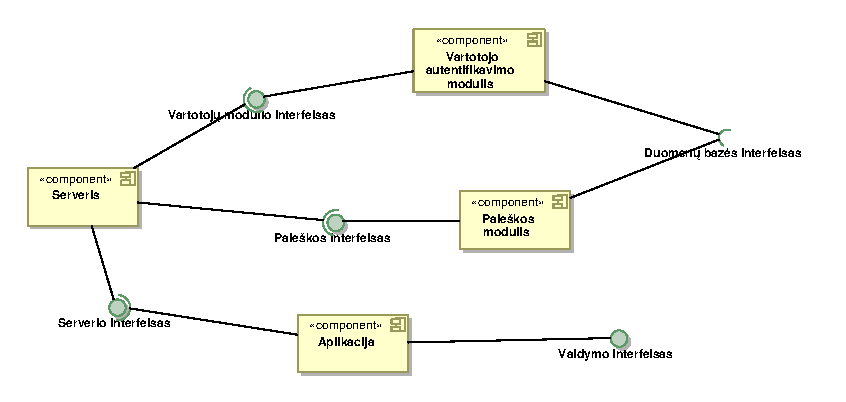
\includegraphics[width=\textwidth]{Komponentai3.eps}
			\caption{Sistemos branduolio komponento dekompozicija\label{Components3}}
		\end{center}
	\end{figure}

	 \bigbreak Jį sudarantys komponentai:\bigbreak
	
	\textbf{Vartotojo autentifikavimo modulis} - šis komponentas vykdo vartotojų autetifikaciją. Jo funkcijos: vartotojų registravimas, prisijungimas.
	
	\textbf{Paieškos modulis} - komponentas, pagal tam tikrus nurodytus kriterijus surandantis skelbimus.
	
	\textbf{Serveris} - komponentas, valdantis prieigą prie duomenų.
	
	\textbf{Aplikacija} - komponentas, kuris pateikia vartotojui skelbimų sąrašą, konkrečių skelbimų detalesnę informaciją.
	\pagebreak

	\section{Dinaminis programų sistemos modelis}
	Šiame skyriuje parodota, kaip vyksta šios sistemos veiksmai bei aprašytos kai kurios galimos vartotojų užduotys. 
	
	\subsection{Vartotojo registracijos veiklos diagrama}
	Procesai, vykstantys vartotojo registracijos metu, parodyti \ref{RegisterActivity} paveikslėlyje. Registravimas vyksta tada, kai vartotojas įsijungia aplikaciją ir pasirenka „Registracija“. Tada vartotojui suvedus reikiamus duomenis sistema patikrina, ar viskas užpildyta teisingai. Jei ne, vartotojas gali bandyti vesti informaciją iš naujo arba išeiti iš registravimosi lango. Jei informacija užpildyta teisingai, vartotojas gali toliau naudotis aplikacija arba išeiti iš jos.
	\begin{figure}[h]
		\begin{center}
			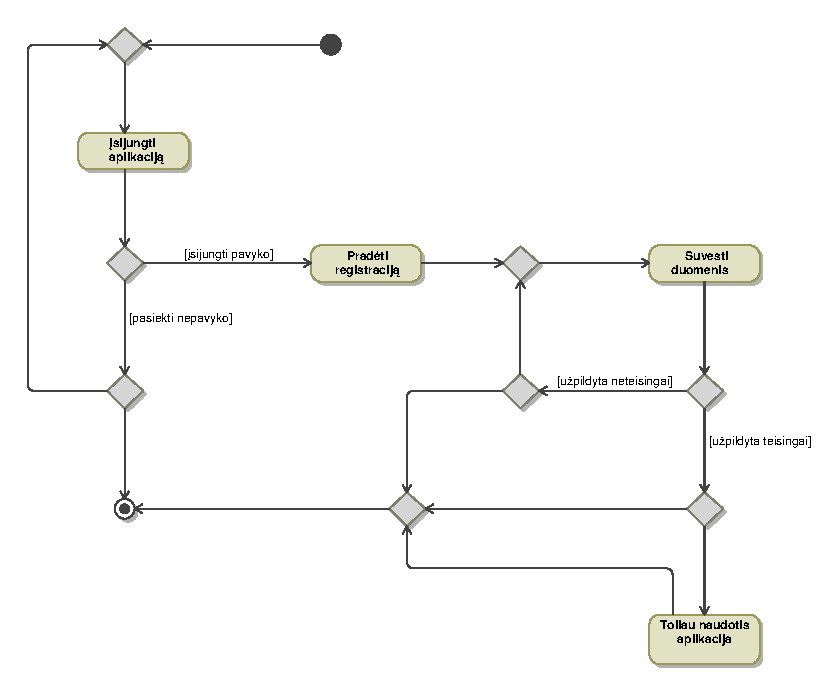
\includegraphics[width=0.85\textwidth]{RegistracijosVeikla.eps}
			\caption{Vartotojo registracijos veiklos diagrama\label{RegisterActivity}}
		\end{center}
	\end{figure}
	
	\pagebreak
	
	\subsection{Skelbimų paieškos veiklos diagrama}
	Procesai, vykstantys skelbimo ieškojimo metu, parodyti \ref{SearchActivity} paveikslėlyje. Pagrindiniame lange vartotojas turi įvesti filtrus, pagal kuriuos bus ieškomi skelbimai. Sistema patikrina, ar įvesti kriterijai yra teisingai suvesti. Jei įvesta klaidingai, vartotojai gali bandyti iš naujo suvesti paieškos kriterijus arba išeiti iš programos. Jei paieškos kriterijai įvesti teisingai, sistema ieško skelbimų. Jei rezultatų nėra, galima pasirinkti kitokius filtrus arba išeiti iš programos. Suradus rezultatų, vartotojas gali pasirinkti skelbimą. Jei jo negalima atidaryti, galima bandyti paiešką atlikti iš naujo. Jei galima atidaryti, vartotojas gali atidaryti skelbimą ir po to grįžti į aplikaciją.
	\begin{figure}[h]
		\begin{center}
			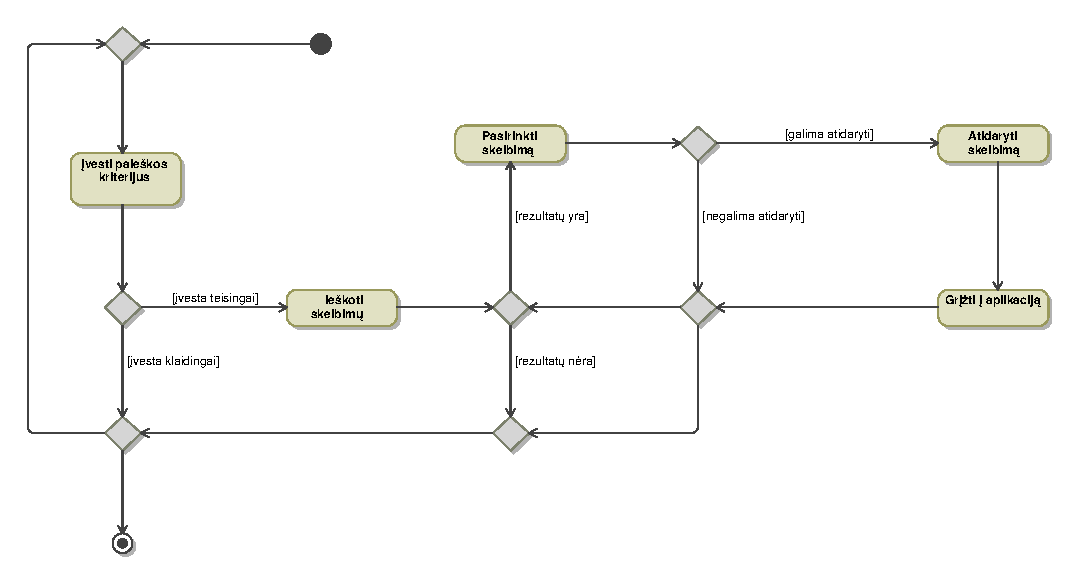
\includegraphics[width=\textwidth]{PaieskosVeikla.eps}
			\caption{Skelbimų paieškos veiklos diagrama\label{SearchActivity}}
		\end{center}
	\end{figure}
	
	\pagebreak
	
	\subsection{Naujo mėgstamo skelbimo veiklos diagrama}
	Procesai, vykstantys vartotojui norint įtraukti skelbimą į mėgstamiausių sąrašą, parodyti \ref{FavActivity} paveikslėlyje. Pirmiausia vartotojas turi prisijungti. Jei to padaryti nepavyksta, jis gali bandyti iš naujo arba išeiti iš programos. Prisijungęs prie sistemos vartotojas ieško jam patinkančio skelbimo ir jį suradęs gali įtraukti į mėgstamiausiųjų sąrašą, o po to ieškoti naujo skelbimo arba išeiti iš šito lango. Jei patinkančio skelbimo vartotojas neranda, tai gali bandyti ieškoti iš naujo arba išeiti iš šito lango.
	\begin{figure}[h]
		\begin{center}
			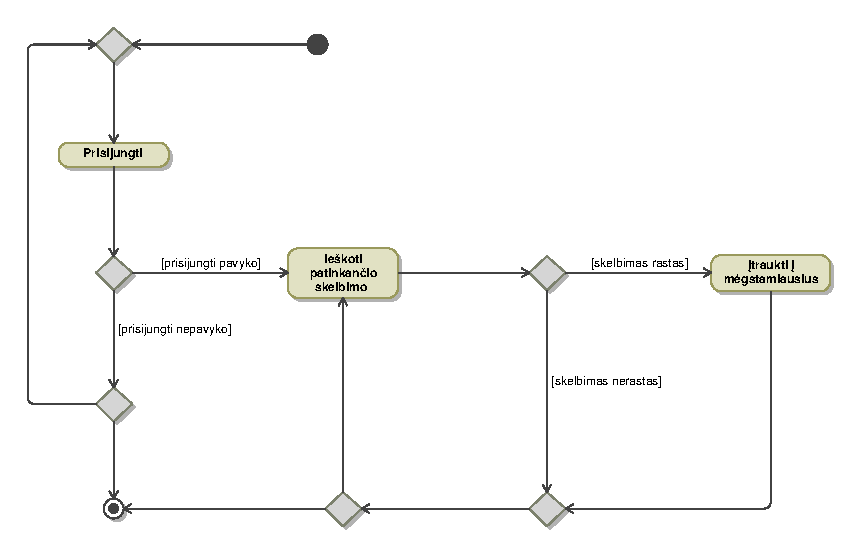
\includegraphics[width=\textwidth]{MegstamiausiuVeikla.eps}
			\caption{Naujo mėgstamo skelbimo veiklos diagrama\label{FavActivity}}
		\end{center}
	\end{figure}
	
	\pagebreak
	
	\section{Komponentų išskirstymas tinkle}
	Šiame skyriuje parodytas sistemos komponentų išdėstymas tinkle.
	\subsection{Komponentų ryšių su artifaktais diagrama}
	
	Žemiau pateiktame komponentų ryšių su artifaktais \ref{ArtComp} paveikslėlyje yra išskirti pagrindiniai sistemos artifaktai. Artifaktus ir komponentus tarpusavyje sieja manifestacijos ryšys. Tai reiškia, kad artifakto sudaromoji dalis yra konkretus komponentas.
	
	\begin{figure}[h]
		\begin{center}
			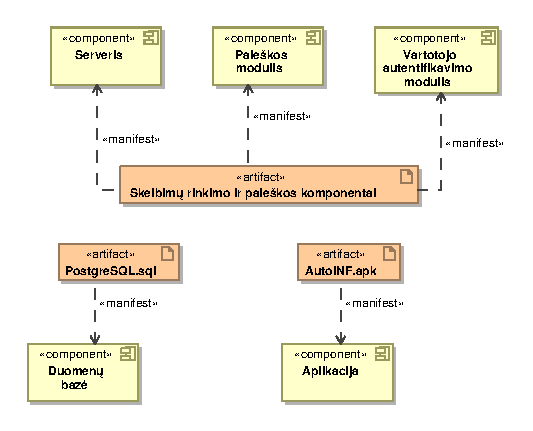
\includegraphics[width=0.8\textwidth]{ArtifaktaiKomponentai.eps}
			\caption{Komponentų ryšių su artifaktais diagrama\label{ArtComp}}
		\end{center}
	\end{figure}

	\begin{indent}
	Sistema susidaro iš trijų pagrindinių dalių - aplikacijos, skelbimų rinkimo ir paieškos komponentų, bei duomenų bazės. Informacijai saugoti apie vartotojų paskyras pasirinkta\break PostgreSQL duomenų bazė.
	\end{indent}
	\pagebreak
	
	\subsection{Diegimo diagrama}
	
	Žemiau pateiktame \ref{Cube} paveikslėlyje yra išskirti fiziniai įrenginiai, rekalingi sistemos darbo palaikymui, bei artifaktų pasiskirstymas tarp jų.\\
	
	\begin{figure}[h]
		\begin{center}
			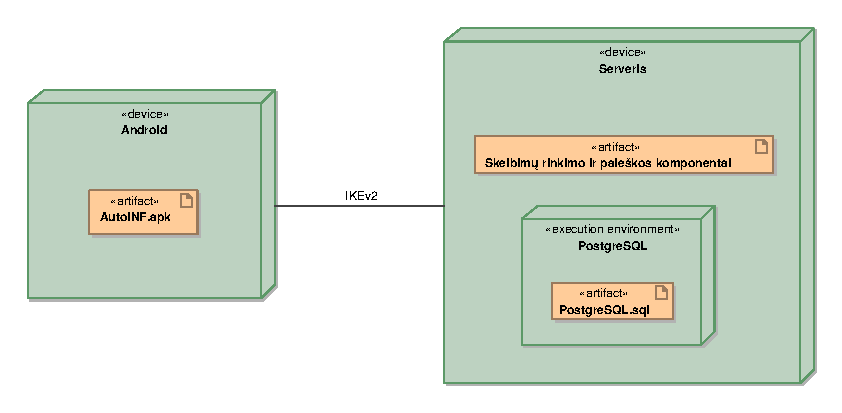
\includegraphics[width=0.9\textwidth]{Mazgai.eps}
			\caption{Diegimo diagrama\label{Cube}}
		\end{center}
	\end{figure}
	
	Beveik visa sistema yra laikoma serveryje. Šiame serveryje yra sudiegiami skelbimų rinkimo ir paieškos komponentai. Tame pačiame serveryje yra ir PostgreSQL duomenų bazė. Vartotojui, norinčiam naudotis sistema iš mobiliojo įrenginio, kuriame yra likusi sistemos dalis, siunčiama užklausa IKEv2 protokolu siekiant gauti sistemos failus.
	\pagebreak	
	
	
	
\renewcommand{\thesubsection}{FR\arabic{subsection}}
\renewcommand*{\theenumi}{\thesubsection.\arabic{enumi}}
\renewcommand*{\theenumii}{\thesubsubsection.\theenumi.\arabic{enumii}}

%\titleformat{\subsection}{\Large\bfseries}{\arabic{subsection}}{1em}{}
\titleformat{\subsubsection}{\bfseries}{\thesubsection.\arabic{subsubsection}}{1em}{}	
	
	
	
	\part*{Reikalavimai}
	\addcontentsline{toc}{part}{Reikalavimai}
	
	Šioje dalyje specifikuojami sistemai taikomi funkciniai, nefunkciniai bei interfeiso reikalavimai.
	
	\setcounter{section}{0}
	\section*{Funkciniai reikalavimai}
	\addcontentsline{toc}{section}{Funkciniai reikalavimai}
	
	\setcounter{subsection}{0}
	\subsection{Bendri reikalavimai}
	\begin{enumerate}[labelindent=10pt,leftmargin=2.2cm]
		\item Įrenginys, kuriame naudojama programinė sistema, turi turėti prieigą prie interneto.
		\item Programinės įrangos įdiegimas laisvai prieinamas visiems norintiems ja naudotis.
		\item Vartotojas turi galimybę keisti savo asmeninius duomenis (vartotojo vardą, el. paštą bei slaptažodį).
		%\item Kiekvieno vartotojo skelbimai, pridėti prie jo mėgstamiausių sąrašo, yra saugomi vartotojo įrenginyje.
		\item Valiutų kursai nustatomi remiantis Lietuvos Banko duomenimis.
		\item Sistema vartotojui neprisijungus leidžia atlikti jos pagrindinę funkciją (skelbimų paieška).
		\item Sistema vartotojui prisijungus leidžia atlikti pagrindinę funkciją (skelbimų paieška) ir papildomą funkciją (skelbimų saugojimas mėgstamiausių sąraše).
		\item Mėgstamiausių sąrašas kiekvienam vartotojui yra prieinamas tik jam ir niekam kitam.
		%\item Sistema vartotojui leidžia iš bet kurio jos lango grįžti į pagrindinį langą.
	\end{enumerate}
	\pagebreak
	
	\renewcommand*{\theenumi}{\thesubsubsection.\arabic{enumi}}
	\renewcommand*{\theenumii}{\thesubsubsection.\theenumi.\arabic{enumii}}
	\renewcommand*{\theenumiii}{\thesubsubsection.\theenumi.\theenumii.\arabic{enumiii}}
	\subsection{Vartotojo užduočių reikalavimai}\label{Vartotojo_reikalavimai}
	Šiame skyriuje nagrinėjami vartotojui aktualūs reikalavimai sistemai „AutoINF“. Pateikiami vartotojo funkciniai reikalavimai, užduočių scenarijai bei jų plėtiniai.
	
	\begin{figure}[h]
		\begin{center}
			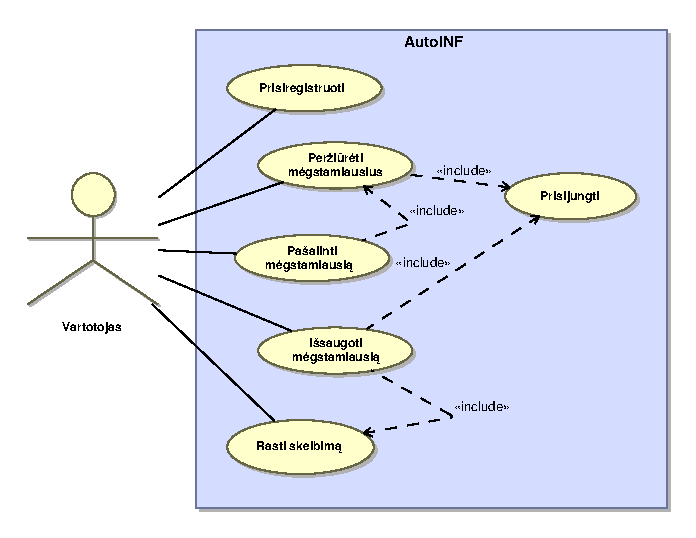
\includegraphics[width=0.7\textwidth]{TikslaiVartotojas.eps}
			\caption{Sistemos užduočių diagrama iš vartotojo perspektyvos\label{UseCaseUser2}}
		\end{center}
	\end{figure}
	\pagebreak
	
	\subsubsection{Pagrindinio meniu reikalavimai}
	\begin{enumerate}[labelindent=10pt,leftmargin=2.2cm]
		\item Pagrindiniame lange vartotojas, jei jis neprisijungęs, turi galimybę pasinaudoti šiomis sistemos funkcijomis: prisiregistruoti, prisijungti bei ieškoti skelbimų.
	\end{enumerate}
		
		\begin{center}
		\captionof{table}{Pagrindinio lango scenarijus, kai vartotojas nėra prisijungęs\label{UserNotLoggedIn}}
		\begin{tabular}{ | c | c | c | }
			\hline
			Žingsnis & Aktorius   & Veiklos apibūdinimas \\ \hline
			1        & Aplikacija & \makecell{Paprašo pasirinkti norimą veiksmą: \\ Prisiregistruoti \\ Prisijungti \\ Rasti skelbimą} \\ \hline
			2        & Vartotojas & Pasirenka veiksmą \\ \hline
			3        & Aplikacija & Įvykdo pasirinktą veiksmą \\ \hline
		\end{tabular}
		\bigskip
		\end{center}
		
	\begin{enumerate}[resume, labelindent=10pt,leftmargin=2.2cm]
		\item Pagrindiniame lange vartotojas, jei jis prisijungęs, turi galimybę pasinaudoti šiomis sistemos funkcijomis: ieškoti skelbimų, peržiūrėti mėgstamiausius.
	\end{enumerate}
		
		\begin{center}
		\captionof{table}{Pagrindinio lango scenarijus, kai vartotojas yra prisijungęs\label{UserLoggedIn}}		
		\begin{tabular}{ | c | c | c | }
			\hline
			Žingsnis & Aktorius   & Veiklos apibūdinimas \\ \hline
			1        & Aplikacija & \makecell{Paprašo pasirinkti norimą veiksmą: \\ Peržiūrėti mėgstamiausius \\ Pašalinti mėgstamiausią \\ Išsaugoti mėgstamiausią \\ Rasti skelbimą} \\ \hline
			2        & Vartotojas & Pasirenka veiksmą \\ \hline
			3        & Aplikacija & Įvykdo pasirinktą veiksmą \\ \hline
		\end{tabular}
		\end{center}		
	\pagebreak
	
	\subsubsection{Vartotojo registracijos reikalavimai}
	\begin{enumerate}[labelindent=10pt,leftmargin=2.2cm]
		\item Sėkmingos registracijos atveju sistema vykdo \ref{UserRegScen} lentelėje nurodytą veiksmų seką.
	\end{enumerate}
		
		\begin{center}
		\captionof{table}{Vartotojo registracijos pagrindinis scenarijus\label{UserRegScen}}		
		\begin{tabular}{ | c | c | c | }
			\hline
			Žingsnis & Aktorius     & Veiklos apibūdinimas \\ \hline
			1        & Vartotojas   & Pasirenka registraciją \\ \hline
			2        & Aplikacija   & Atidaro registracijos langą \\ \hline
			3        & Vartotojas   & \makecell{Suveda prisiregistravimo duomenis ir \\ spaudžia mygtuką „Prisiregistruoti“} \\ \hline
			4        & Aplikacija   & Validuoja duomenis ir siunčia užklausą į serverį \\ \hline
			5        & Serveris     & Siunčia užklausą į duomenų bazę \\ \hline
			6        & Duomenų bazė & \makecell{Išsaugo naujos paskyros duomenis ir \\ perspėja serverį apie sėkmingą registraciją} \\ \hline
			7        & Serveris     & Perspėja aplikaciją apie sėkmingą registraciją \\ \hline
			8        & Aplikacija   & \makecell{Parodo pranešimą apie registracijos sėkmingumą, \\ perkrauna pagrindinį langą su prisijungusio vartotojo \\ interfeisu ir laukia, kol vartotojas atliks kitą veiksmą} \\ \hline
		\end{tabular}
		\end{center}
		\bigskip
		
	\begin{enumerate}[resume, labelindent=10pt,leftmargin=2.2cm]
		\item Nesėkmingos registracijos atveju sistema į klaidas reaguoja pagal \ref{UserRegScenExtra} lentelę.
	\end{enumerate}
		
		\begin{center}
		\captionof{table}{Vartotojo registracijos scenarijaus plėtiniai\label{UserRegScenExtra}}		
		\begin{tabular}{ | c | c | c | }
			\hline
			Žingsnis & Sąlyga & Veiklos apibūdinimas \\ \hline
			4a       & \makecell{Vartotojo duomenų \\ validacija nesėkminga} & \makecell{Klaidingai užpildyti (neužpildyti) laukai yra paryškinami \\ raudonai ir lango viršuje parodomas tekstas, kad kai \\ kurie laukai yra užpildyti klaidingai (neužpildyti)} \\ \hline
			6a       & \makecell{Duomenų bazėje \\ nepavyko išsaugoti \\ duomenų} & Parodomas pranešimas apie nesėkmingą registraciją \\ \hline
		\end{tabular}
		\end{center}
		\pagebreak
		
	\begin{enumerate}[resume, labelindent=10pt,leftmargin=2.2cm]
		\item\label{Validation} Vartotojui patvirtinus registraciją sistema turi validuoti vartotojo įvestus duomenis:
		
		\begin{enumerate}[label=\theenumi.\arabic{enumii}]
			\item Visi privalomi laukai (vartotojo vardas, el. paštas bei slaptažodis) turi būti užpildyti.
			\item Galimi simboliai: lotyniškos mažosios bei didžiosios raidės, skaičiai.
			\item El. pašto lauko įvestis turi būti formato „pavyzdys@mail.lt“.
			\item Slaptažodį turi sudaryti bent 8 simboliai, tarp kurių yra bent viena mažoji raidė, didžioji raidė ir bent vienas skaičius.
		\end{enumerate}	
		
		\item Prieš sukurdama naują paskyrą sistema turi užtikrinti, kad dar neegzistuoja paskyra su įvestu vartotojo vardu ar el. paštu.
		\item Vartotojo vardas ir el. paštas duomenų bazėje saugomi simbolių eilutės („string“) formatu, o slaptažodžiui pritaikoma maišos („hash“) funkcija.
	\end{enumerate}	
	\pagebreak
	
	\subsubsection{Vartotojo prisijungimo reikalavimai\label{LogInLabel}}
	\begin{enumerate}[labelindent=10pt,leftmargin=2.2cm]
		\item Sėkmingo prisijungimo atveju sistema vykdo \ref{UserLogInScen} lentelėje nurodytą veiksmų seką.
	\end{enumerate}
		
		\begin{center}
		\captionof{table}{Vartotojo prisijungimo pagrindinis scenarijus\label{UserLogInScen}}		
		\begin{tabular}{ | c | c | c | }
			\hline
			Žingsnis & Aktorius     & Veiklos apibūdinimas \\ \hline
			1        & Vartotojas   & Pasirenka prisijungimo funkciją \\ \hline
			2        & Aplikacija   & Parodo prisijungimo langą \\ \hline
			3        & Vartotojas   & \makecell{Įveda prisijungimo duomenis ir \\ spaudžia mygtuką „Prisijungti“} \\ \hline
			4        & Aplikacija   & Validuoja duomenis ir siunčia užklausą į serverį \\ \hline
			5        & Serveris     & Siunčia užklausą į duomenų bazę \\ \hline
			6        & Duomenų bazė & \makecell{Patikrina, ar tokia paskyra egzistuoja ir \\ praneša serveriui apie sėkmingą prisijungimą} \\ \hline
			7        & Serveris     & Praneša aplikacijai apie sėkmingą prisijungimą \\ \hline
			8        & Aplikacija   & \makecell{Parodo pagrindinį langą su papildomomis \\ prisijungusio vartotojo funkcijomis} \\ \hline
		\end{tabular}
		\bigskip
		\end{center}
		
	\begin{enumerate}[resume, labelindent=10pt,leftmargin=2.2cm]
		\item Nesėkmingo prisijungimo atveju sistema į klaidas reaguoja pagal \ref{UserLogInScenExtra} lentelę.
	\end{enumerate}		
		
		\begin{center}
		\captionof{table}{Vartotojo prisijungimo scenarijaus plėtiniai\label{UserLogInScenExtra}}		
		\begin{tabular}{ | c | c | c | }
			\hline
			Žingsnis & Sąlyga & Veiklos apibūdinimas \\ \hline
			4a       & \makecell{Įvestų duomenų \\ validacija nesėkminga} & \makecell{Klaidingai užpildyti (neužpildyti) laukai yra paryškinami \\ raudonai ir lango viršuje parodomas tekstas, kad kai \\ kurie laukai yra užpildyti klaidingai (neužpildyti)} \\ \hline
			6a       & \makecell{Suvesti klaidingi \\ prisijungimo duomenys} & \makecell{Parodomas pranešimas apie paskyros \\ neegzistavimą / klaidingą slaptažodį} \\ \hline
		\end{tabular}
		\end{center}
	\pagebreak
	
	\begin{enumerate}[resume, labelindent=10pt,leftmargin=2.2cm]
		\item Prisijungimo duomenų validacija tokia pati kaip ir \ref{Validation} punkte nurodyta registracijos metu vykdoma validacija (išskyrus prisijungimui nenaudojamą el. paštą).
		\item Slaptažodis lyginamas su rastos paskyros slaptažodžiu iš pradžių pritaikius maišos („hash“) funkciją.
	\end{enumerate}
	\pagebreak
	
	\subsubsection{Vartotojo skelbimų paieškos reikalavimai}
	\begin{enumerate}[labelindent=10pt,leftmargin=2.2cm]
		\item Sėkmingos paieškos atveju sistema vykdo \ref{UserSearchScen} lentelėje nurodytą veiksmų seką.
	\end{enumerate}
		
		\begin{center}
		\captionof{table}{Vartotojo skelbimų ieškojimo pagrindinis scenarijus\label{UserSearchScen}}		
		\begin{tabular}{ | c | c | c | }
			\hline
			Žingsnis & Aktorius     & Veiklos apibūdinimas \\ \hline
			1        & Vartotojas   & \makecell{Vartotojas įveda paieškos kriterijus \\ ir spaudžia mygtuką „Ieškoti“} \\ \hline
			2        & Aplikacija   & Siunčia užklausą į serverį \\ \hline
			3        & Serveris     & Siunčia užklausą į paieškos modulį \\ \hline
			4        & Paieškos modulis & \makecell{Randa skelbimus, atitinkančius vartotojo \\ nurodytus kriterijus ir grąžina juos serveriui} \\ \hline
			5        & Serveris     & Grąžina aplikacijai rastus skelbimus  \\ \hline
			6        & Aplikacija   & Parodo rastų skelbimų sąrašą \\ \hline
			7        & Vartotojas   & Paspausžia ant skelbimo \\ \hline
			8        & Aplikacija   & Atidaro skelbimo langą \\ \hline
		\end{tabular}
		\end{center}
		\bigskip

	\begin{enumerate}[resume,labelindent=10pt,leftmargin=2.2cm]
		\item Nesėkmingos paieškos atveju sistema į klaidas reaguoja pagal \ref{UserSearchScenExtra} lentelę.
	\end{enumerate}

		\begin{center}
		\captionof{table}{Vartotojo skelbimų ieškojimo scenarijaus plėtiniai\label{UserSearchScenExtra}}		
		\begin{tabular}{ | c | c | c | }
			\hline
			Žingsnis & Sąlyga & Veiklos apibūdinimas \\ \hline
			1a       & \makecell{Vartotojas nesuveda \\ privalomų paieškos kriterijų} & \makecell{Vartotojas įspėjamas, kad negalima \\ palikti neužpildytų privalomų laukų} \\ \hline
			5a       & Nerasta skelbimų & \makecell{Parodomas pranešimas, kad nėra skelbimų, \\ atitinkančių nurodytą filtrą, ir vartotojas yra \\ grąžinamas į pagrindinį (paieškos) langą } \\ \hline
			7a       & \makecell{Vartotojas nepaspaudžia \\ ant skelbimo} & \makecell{Aplikacija laukia, kol bus paspausta ant \\ skelbimo arba kol vartotojas ieškos naujų \\ skelbimų pagal kitą filtrą} \\ \hline
		\end{tabular}
		\end{center}
		\pagebreak
		
	\begin{enumerate}[resume,labelindent=10pt,leftmargin=2.2cm]
		\item Pradėdama paiešką sistema filtruoja skelbimų šaltinius:
		
		\begin{enumerate}[label=\theenumi.\arabic{enumii}]
			\item Jei nurodyti ieškomų transporto priemonių tipai, imami tik tie šaltiniai, kuriuose yra šių tipų transporto priemonių skelbimai.
			\item Jei nurodytos valstybės, imami tik tie šaltiniai, kuriuose talpinami tose valstybėse skelbiamų transporto priemonių skelbimai.
		\end{enumerate}				
		
		\item Ieškodama skelbimų, sistema iš kiekvieno tinkančio skelbimų šaltinio gauna visus skelbimus ir rodo tik tuos, kurie atitinka visus vartotojo nurodytus kriterijus.
		
	\end{enumerate}
	\pagebreak
	
	\subsubsection{Vartotojo mėgstamiausių skelbimų peržiūros reikalavimai}
	\begin{enumerate}[labelindent=10pt,leftmargin=2.2cm]
		\item Sėkmingos mėgstamiausių skelbimų peržiūros atveju sistema vykdo \ref{UserViewFavScen} lentelėje nurodytą veiksmų seką.
	\end{enumerate}
		
		\begin{center}
		\captionof{table}{Vartotojo mėgstamiausių skelbimų peržiūros pagrindinis scenarijus\label{UserViewFavScen}}		
		\begin{tabular}{ | c | c | c | }
			\hline
			Žingsnis & Aktorius     & Veiklos apibūdinimas \\ \hline
			1        & Vartotojas   & Pasirenka „Peržiūrėti mėgstamiausius“ funkciją \\ \hline
			2        & Aplikacija   & Siunčia užklausą į serverį \\ \hline
			3        & Serveris     & Siunčia užklausą į duomenų bazę \\ \hline
			4        & Duomenų bazė & Siunčia serveriui vartotojo mėgstamiausių skelbimų URL kodus \\ \hline
			5        & Serveris     & Siunčia aplikacijai vartotojo mėgstamiausių skelbimų sąrašą \\ \hline
			6        & Aplikacija   & \makecell{Atidaro naują langą su vartotojo išsaugotais \\ jo mėgstamiausiais skelbimais } \\ \hline
		\end{tabular}
		\end{center}
		\bigskip
		
	\begin{enumerate}[resume,labelindent=10pt,leftmargin=2.2cm]
		\item Duomenų bazė serveriui grąžina URL kodus.
		\item Serveris URL kodus paverčia skelbimais, kuriuos geba vaizduoti aplikacija.
	\end{enumerate}
	\pagebreak
	
	\subsubsection{Vartotojo mėgstamiausio skelbimo išsaugojimo reikalavimai}
	\begin{enumerate}[labelindent=10pt,leftmargin=2.2cm]
		\item Sėkmingo mėgstamiausio skelbimo išsaugojimo atveju sistema vykdo \ref{UserSaveAdScen} lentelėje nurodytą veiksmų seką.
	\end{enumerate}
		
		\begin{center}
		\captionof{table}{Vartotojo mėgstamiausio skelbimo išsaugojimo pagrindinis scenarijus\label{UserSaveAdScen}}		
		\begin{tabular}{ | c | c | c | }
			\hline
			Žingsnis & Aktorius         & Veiklos apibūdinimas \\ \hline
			1        & Vartotojas       & Vykdo skelbimų paiešką \\ \hline
			2        & Aplikacija       & Siunčia užklausą į serverį \\ \hline
			3        & Serveris         & Siunčia užklausą į paieškos modulį \\ \hline
			4        & Paieškos modulis & Grąžina serveriui paieškos rezultatus \\ \hline
			5        & Serveris         & Grąžina aplikacijai paieškos rezultatus  \\ \hline
			6        & Aplikacija       & Parodo rastų skelbimų sąrašą \\ \hline
			7        & Vartotojas       & Prideda norimą skelbimą prie mėgstamiausių \\ \hline
			8        & Aplikacija       & Siunčia užklausą į serverį \\ \hline
			9        & Serveris         & Siunčia užklausą į duomenų bazę \\ \hline
			10       & Duomenų bazė     & \makecell{Išsaugo skelbimą mėgstamiausių sąraše ir \\ praneša serveriui apie sėkmingą skelbimo išsaugojimą} \\ \hline
			11       & Serveris         & Praneša aplikacijai apie sėkmingą skelbimo išsaugojimą \\ \hline
			12       & Aplikacija       & Praneša apie sėkmingą skelbimo išsaugojimą \\ \hline
		\end{tabular}
		\end{center}
		\bigskip
		
	\begin{enumerate}[resume,labelindent=10pt,leftmargin=2.2cm]
		\item Mėgstamiausio skelbimo išsaugojimo funkcija vartotojui turi būti prieinama tik prieš tai atlikus skelbimų paiešką.
		\item Duomenų bazėje skelbimai saugomi URL kodu.
		\item Išsaugojimo metu duomenų bazėje saugomas vartotojo mėgstamiausių skelbimų sąrašas keičiamas esamu sąrašu, papildytu išsaugojamu skelbimu.
	\end{enumerate}
	\pagebreak
	
	\subsubsection{Vartotojo mėgstamiausio skelbimo pašalinimo reikalavimai}
	\begin{enumerate}[labelindent=10pt,leftmargin=2.2cm]
		\item Sėkmingo mėgstamiausio skelbimo pašalinimo atveju sistema vykdo \ref{UserRemoveAdScen} lentelėje nurodytą veiksmų seką.
	\end{enumerate}
		
		\begin{center}
		\captionof{table}{Vartotojo mėgstamiausio skelbimo pašalinimo pagrindinis scenarijus\label{UserRemoveAdScen}}
		\begin{tabular}{ | c | c | c | }
			\hline
			Žingsnis & Aktorius       & Veiklos apibūdinimas \\ \hline
			1        & Vartotojas     & Pasirenka „Peržiūrėti mėgstamiausius“ \\ \hline
			2        & Aplikacija     & Parodo mėgstamiausių sąrašą \\ \hline
			3        & Vartotojas     & Pasirenka skelbimo šalinimą \\ \hline
			4        & Aplikacija     & Siunčia užklausą į serverį \\ \hline
			5        & Serveris       & Siunčia užklausą į duomenų bazę  \\ \hline
			6        & Duomenų bazė   & \makecell{Pašalina mėgstamiausią skelbimą ir grąžina \\ pranešimą apie sėkmingai pašalintą skelbimą} \\ \hline
			7        & Serveris       & \makecell{Grąžina pranešimą apie sėkmingai \\ pašalintą mėgstamiausią skelbimą} \\ \hline
			8        & Aplikacija     & Atnaujina mėgstamiausių skelbimų sąrašą \\ \hline
		\end{tabular}
		\end{center}
		\bigskip

	\begin{enumerate}[resume,labelindent=10pt,leftmargin=2.2cm]
		\item Nesėkmingo mėgstamiausio skelbimo pašalinimo atveju sistema į klaidas reaguoja pagal \ref{UserRemoveAdExtra} lentelę.
	\end{enumerate}	

		\begin{center}
		\captionof{table}{Vartotojo mėgstamiausio skelbimo pašalinimo scenarijaus plėtiniai\label{UserRemoveAdExtra}}		
		\begin{tabular}{ | c | c | c | }
			\hline
			Žingsnis & Sąlyga & Veiklos apibūdinimas \\ \hline
			6a       & \makecell{Nepavyko pašalinti \\ skelbimo iš \\ duomenų bazės} & \makecell{Grąžina pranešimą apie nesėkmingą \\ skelbimo pašalinimą iš duomenų bazės} \\ \hline
		\end{tabular}
		\end{center}
		\bigskip
		
	\begin{enumerate}[resume,labelindent=10pt,leftmargin=2.2cm]
		\item Mėgstamiausio skelbimo pašalinimo funkcija vartotojui turi būti prieinama tik prieš tai atlikus mėgstamiausių skelbimų peržiūrą.
		\item Vartotojui pasirinkus mėgstamiausio skelbimo šalinimą, sistema parodo naują langą, kuriame vartotojas turi patvirtinti savo sprendimą.
		\item Šalinimo metu duomenų bazėje saugomas vartotojo mėgstamiausių skelbimų sąrašas keičiamas esamu sąrašu be šalinamo skelbimo.
	\end{enumerate}		
	\pagebreak	
	
	\subsection{Administratoriaus užduočių reikalavimai}
	Šiame skyriuje nagrinėjami administratoriui aktualūs reikalavimai sistemai „AutoINF“. Pateikiami administratoriaus funkciniai reikalavimai, užduočių scenarijai bei jų plėtiniai.
	
	\begin{figure}[h]
		\begin{center}
			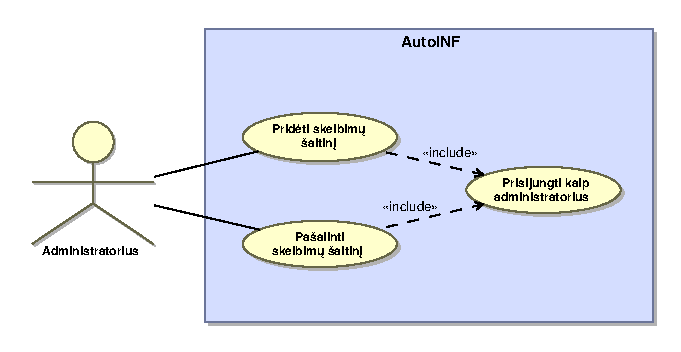
\includegraphics[width=0.7\textwidth]{TikslaiAdministratorius.eps}
			\caption{Sistemos užduočių diagrama iš administratoriaus perspektyvos\label{UseCaseAdmin2}}
		\end{center}
	\end{figure}
	\pagebreak
	
	\subsubsection{Administratoriaus prisijungimo reikalavimai}
	\begin{enumerate}[labelindent=10pt,leftmargin=2.2cm]
		\item Administratoriaus prisijungimui taikomi visi reikalavimai, nurodyti \ref{LogInLabel} skyriuje.
		\item Sistema papildomai turi patikrinti, ar paskyra, prie kurios jungiamasi, yra administratoriaus paskyra.
	\end{enumerate}
		
		\begin{center}
		\captionof{table}{Pagrindinio lango scenarijus, kai administratorius yra prisijungęs\label{AdmindLoggedIn}}		
		\begin{tabular}{ | c | c | c | }
			\hline
			Žingsnis & Aktorius         & Veiklos apibūdinimas \\ \hline
			1        & Aplikacija       & \makecell{Aplikacija paprašo pasirinkti norimą veiksmą: \\ Pridėti skelbimų šaltinį \\ Pašalinti skelbimų šaltinį} \\ \hline
			2        & Administratorius & Administratorius pasirenka veiksmą \\ \hline
			3        & Aplikacija       & Aplikacija įvykdo pasirinktą veiksmą \\ \hline
		\end{tabular}
		\end{center}
		\bigskip
		
	\begin{enumerate}[resume,labelindent=10pt,leftmargin=2.2cm]
		\item Po sėkmingo administratoriaus prisijungimo sistema visada vykdo \ref{AdminViewSourcesScen} lentelėje pavaizduotą skelbimų šaltinių peržiūros funkciją.
	\end{enumerate}

		\begin{center}
		\captionof{table}{Administratoriaus skelbimų šaltinių peržiūros pagrindinis scenarijus\label{AdminViewSourcesScen}}
		\begin{tabular}{ | c | c | c | }
			\hline
			Žingsnis & Aktorius         & Veiklos apibūdinimas \\ \hline
			1        & Administratorius & Prisijungia \\ \hline
			2        & Aplikacija       & Siunčia užklausą į serverį \\ \hline
			3        & Serveris         & Siunčia užklausą į duomenų bazę \\ \hline
			4        & Duomenų bazė     & Grąžina skelbimų šaltinių sąrašą į serverį \\ \hline
			5        & Serveris         & Grąžina skelbimų šaltinių sąrašą į aplikaciją \\ \hline
			6        & Aplikacija       & Parodo skelbimų šaltinių sąrašą \\ \hline
		\end{tabular}
		\end{center}
		\pagebreak
	
	\begin{enumerate}[resume,labelindent=10pt,leftmargin=2.2cm]
		\item Nesėkmingo skelbimų šaltinių peržiūros atveju sistema į klaidas reaguoja pagal \ref{AdminViewSourcesScenExtra} lentelę.
	\end{enumerate}
	
		\begin{center}
		\captionof{table}{Administratoriaus skelbimų šaltinių peržiūros scenarijaus plėtiniai\label{AdminViewSourcesScenExtra}}		
		\begin{tabular}{ | c | c | c | }
			\hline
			Žingsnis & Sąlyga         & Veiklos apibūdinimas \\ \hline
			4a       & \makecell{Duomenų bazėje \\ nėra šaltinių} & \makecell{Duomenų bazė grąžina pranešimą, kad \\ skelbimų šaltinių nėra} \\ \hline
		\end{tabular}
		\end{center}
		\pagebreak
	
	\subsubsection{Administratoriaus skelbimų šaltinio pridėjimo reikalavimai}
	\begin{enumerate}[labelindent=10pt,leftmargin=2.2cm]
		\item Sėkmingo skelbimų šaltinio pridėjimo atveju sistema vykdo \ref{AdminAddSourceScen} lentelėje nurodytą veiksmų seką.
	\end{enumerate}
		
		\begin{center}
		\captionof{table}{Administratoriaus skelbimų šaltinio pridėjimo pagrindinis scenarijus\label{AdminAddSourceScen}}		
		\begin{tabular}{ | c | c | c | }
			\hline
			Žingsnis & Aktorius         & Veiklos apibūdinimas \\ \hline
			1        & Administratorius & \makecell{Suveda naujo skelbimų šaltinio duomenis ir \\ spaudžia mygtuką „Pridėti šaltinį“ } \\ \hline
			2        & Aplikacija       & Siunčia užklausą į serverį \\ \hline
			3        & Serveris         & Siunčia užklausą į duomenų bazę \\ \hline
			4        & Duomenų bazė     & \makecell{Prideda naują skelbimų šaltinį ir praneša \\ serveriui apie sėkmingą skelbimų šaltinio pridėjimą} \\ \hline
			5        & Serveris         & \makecell{Praneša aplikacijai apie sėkmingą skelbimų \\ šaltinio pridėjimą} \\ \hline
			6        & Aplikacija       & Atnaujina skelbimų šaltinių sąrašą \\ \hline
		\end{tabular}
		\end{center}
		\bigskip

	\begin{enumerate}[resume,labelindent=10pt,leftmargin=2.2cm]
		\item Nesėkmingo skelbimų šaltinio pridėjimo atveju sistema į klaidas reaguoja pagal \ref{AdminAddSourceScenExtra} lentelę.
	\end{enumerate}

		\begin{center}
		\captionof{table}{Administratoriaus skelbimų šaltinio pridėjimo scenarijaus plėtiniai\label{AdminAddSourceScenExtra}}		
		\begin{tabular}{ | c | c | c | }
			\hline
			Žingsnis & Sąlyga         & Veiklos apibūdinimas \\ \hline
			4a       & \makecell{Nepavyksta \\ pridėti šaltinio} & \makecell{Duomenų bazė grąžina pranešimą apie \\ nesėkmingą skelbimų šaltinio pridėjimą} \\ \hline
		\end{tabular}
		\end{center}
		\bigskip
		
	\begin{enumerate}[resume,labelindent=10pt,leftmargin=2.2cm]
		\item Skelbimų šaltinio pridėjimo funkcija administratoriui turi būti prieinama tik prieš tai sistemai atlikus skelbimų šaltinių peržiūros funkciją.
		\item Duomenų bazėje skelbimų šaltinis saugomas tokiu formatu:
		
			\begin{enumerate}[label=\theenumi.\arabic{enumii}]
				\item URL kodas,
				\item Skelbiamų transporto priemonių tipai (pvz., automobiliai, motociklai),
				\item Valstybės, kuriose skelbiamos visos šaltinio skelbimų transporto priemonės.
			\end{enumerate}
		 
	\end{enumerate}
	\pagebreak
	
	\subsubsection{Administratoriaus skelbimų šaltinio pašalinimo reikalavimai}
	\begin{enumerate}[labelindent=10pt,leftmargin=2.2cm]
		\item Sėkmingo skelbimų šaltinio pašalinimo atveju sistema vykdo \ref{AdminRemoveSourceScen} lentelėje nurodytą veiksmų seką.
	\end{enumerate}
		
		\begin{center}
		\captionof{table}{Administratoriaus skelbimų šaltinio pašalinimo pagrindinis scenarijus\label{AdminRemoveSourceScen}}		
		\begin{tabular}{ | c | c | c | }
			\hline
			Žingsnis & Aktorius         & Veiklos apibūdinimas \\ \hline
			1        & Administratorius & Pasirenka skelbimų šaltinio pašalinimą \\ \hline
			2        & Aplikacija       & Siunčia užklausą serveriui \\ \hline
			3        & Serveris         & Siunčia užklausą duomenų bazei \\ \hline
			4        & Duomenų bazė     & \makecell{Pašalina skelbimų šaltinį ir siunčia pranešimą \\ serveriui apie sėkmingai pašalintą skelbimų šaltinį} \\ \hline
			5        & Serveris         & \makecell{Siunčia pranešimą aplikacijai apie \\ sėkmingai pašalintą skelbimų sąrašą} \\ \hline
			6        & Aplikacija       & \makecell{Atnaujina skelbimų sąrašą ir laukia \\ tolimesnių administratoriaus veiksmų} \\ \hline
		\end{tabular}
		\end{center}
		\bigskip

	\begin{enumerate}[resume,labelindent=10pt,leftmargin=2.2cm]
		\item Nesėkmingo skelbimų šaltinio pašalinimo atveju sistema į klaidas reaguoja pagal \ref{AdminRemoveSourceScenExtra} lentelę.
	\end{enumerate}

		\begin{center}
		\captionof{table}{Administratoriaus skelbimų šaltinio šalinimo scenarijaus plėtiniai\label{AdminRemoveSourceScenExtra}}		
		\begin{tabular}{ | c | c | c | }
			\hline
			Žingsnis & Sąlyga         & Veiklos apibūdinimas \\ \hline
			4a       & \makecell{Nepavyksta \\ pašalinti šaltinio} & \makecell{Duomenų bazė grąžina pranešimą apie \\ nesėkmingą skelbimų šaltinio pašalinimą} \\ \hline
		\end{tabular}
		\end{center}
		\bigskip
		
	\begin{enumerate}[resume,labelindent=10pt,leftmargin=2.2cm]
		\item Skelbimų šaltinio pašalinimo funkcija administratoriui turi būti prieinama tik prieš tai sistemai atlikus skelbimų šaltinių peržiūros funkciją.
		\item Administratoriui pasirinkus skelbimų šaltinio šalinimą, sistema parodo naują langą, kuriame administratorius turi patvirtinti savo sprendimą.
	\end{enumerate}
	\pagebreak
	
	\renewcommand{\thesubsection}{NFR\arabic{subsection}}
	\renewcommand*{\theenumi}{\thesubsection.\arabic{enumi}}
	\renewcommand*{\theenumii}{\theenumi.\arabic{enumii}}
	\section*{Nefunkciniai reikalavimai}
	\addcontentsline{toc}{section}{Nefunkciniai reikalavimai}
	\setcounter{subsection}{0}
	
	\subsection{Vidinių interfeisų reikalavimai}
	\begin{enumerate}[labelindent=10pt,leftmargin=2.2cm]
		\item Sistema turi būti suprogramuota Java programavimo kalba.
		\item Sistema sukompiliuota laisvai platinamu standartiniu Java kompiliarotiumi.
		\item Sistema veikia Android aplinkoje, versijos pasirinkimas paliekamas programuotojų nuožiūrai.
		\item Programavimo aplinkos pasirinkimas paliekamas programuotojų nuožiūrai.
		\item Duomenims saugoti naudojama PostgreSQL duomenų bazė.
	\end{enumerate}	
	
	%\renewcommand*{\theenumi}{\thesubsubsection.\arabic{enumi}}
	%\renewcommand*{\theenumii}{\thesubsubsection.\theenumi.\arabic{enumii}}
	%\renewcommand*{\theenumiii}{\thesubsubsection.\theenumi.\theenumii.\arabic{enumiii}}
	%\subsection{Veikimo reikalavimai}
	%Šiame skyriuje aprašomi sistemos veikimo reikalavimai.
	
	\subsection{Tikslumo reikalavimai}
	\begin{enumerate}[labelindent=10pt,leftmargin=2.2cm]
		\item Skelbimo kaina atvaizduojama „double“ formatu 2 skačių po kablelio tikslumu ir nėra apvalinama.
		\item Duomenys apie valiutų kursus saugomi „double“ formatu. Skaičių kiekis po kablelio neribojamas.
	\end{enumerate}	
	
	\subsection{Patikimumo reikalavimai}
	\begin{enumerate}[labelindent=10pt,leftmargin=2.2cm]
		\item Įvykus bet kokiam sistemos sutrikimui, sistema, jei įmanoma, turi perkelti vartotoją į prieš tai atliktą žingsnį.
		\item Įvykus sutrikimui sistema neatskleidžia vidinių sutrikimo priežasčių vartotojui (nebent sutrikimas įvyko dėl jo kaltės). Visus sistemos lūžius ir to priežastis sistema saugo duomenų bazėje, prieinamoje tik savininkui ir administratoriams.
		\item Skelbimas vartotojo mėgstamiausiųjų sąraše atsiranda tik tada, kai jis pridedamas į duomenų bazę.
		\item Sistema nėra galima naudotis, kai atnaujinama sistemos duomenų bazė.
	\end{enumerate}	
	
	\subsection{Robastiškumo reikalavimai}
	\begin{enumerate}[labelindent=10pt,leftmargin=2.2cm]
		\item Visos klaidos yra saugomos sistemos duomenų bazėje, klaidų registre.
		\item Įvykus nedideliam sutrikimui (pvz., dingsta ryšys su duomenų baze; skelbimų šaltiniai nepasiekiami) sistema kartoja paskutinį veiksmą 30 s. Neatsistačius funkcionalumui sistema išsaugo klaidos priežastį duomenų bazėje, atsiprašo vartotojo už nepatogumus ir prašo vartotojo pabandyti naudotis sistema vėliau.
		\item Įvykus rimtam sutrikimui (pvz., atnaujintas skelbimų puslapio HTML kodas; pasikeičia skelbimų nuskaitymo būdas, todėl nebeįmanoma gauti skelbimų informacijos), sistema turi gebėti išimti puslapį iš pasirinkimo galimybių ir užregistruoti veiksmą duomenų bazėje.
		\item Po sistemos sutrikimo tikėtinas atsistatymo laikas yra laikas, reikalingas sistemos perkrovimui.
		\item Sutrikus infrastruktūrai (pvz., duomenų bazei) sistema pradeda veikti iš karto, kai infrastruktūra yra sutvarkyta.
	\end{enumerate}	
	
	\subsection{Našumo reikalavimai}
	\begin{enumerate}[labelindent=10pt,leftmargin=2.2cm]
		\item Sistema vos pradėjusi paiešką turi pranešti vartotojui, kad priėmė paieškos duomenis ir kad paieška yra vykdoma.
		\item Sistema turi parodyti pirmąjį užklausos puslapį ne lėčiau kaip per 10 s.
		\item Sistema į vartotojo įvestį turi sureguoti ne lėčiau kaip per 0,5 s.
		\item Užklausų skaičius, kurį maksimaliai be vėlavimo gali atlikti serveris, yra 10 000 per sekundę (nebent sistemos savininko infrastruktūra nėra pakankamai pajėgi).
	\end{enumerate}
	
	\pagebreak
	\renewcommand{\thesubsection}{IR\arabic{subsection}}
	%\renewcommand*{\theenumi}{IR\arabic{enumi}}
	%\renewcommand*{\theenumii}{\theenumi.\arabic{enumii}}
	\section*{Interfeiso reikalavimai}	
	\addcontentsline{toc}{section}{Interfeiso reikalavimai}
	\setcounter{subsection}{0}	
	\subsection{Bendri reikalavimai}	
	\begin{enumerate}[labelindent=10pt,leftmargin=2.2cm]
		\item Originali valiuta automatiškai vaizduojama eurais, bet vartotojas gali pasirinkti, kurią valiutą iš pagrindinių (pagrindinės valiutos pasirenkamos programuotojų atžvilgiu, bet nemažiau kaip 3, iš kurių viena - euras) rodyti.
		\item\label{MainWindowDisplayReq} Pagrindinis langas, kuris atvaizduojamas įjungus programą, yra paieškos langas.
		\item\label{AdParts} Visi skelbimai sąraše atvaizduojami formatu, kurio pagrindinės dalys yra:
		
		\begin{enumerate}[label=\theenumi.\arabic{enumii}]
			\item Pagrindinė skelbimo nuotrauka,
			\item Transporto priemonės markė,
			\item Transporto priemonės modelis,
			\item Kuro tipas,
			\item Variklio litražas,
			\item Kėbulo tipas,
			\item Valstybė,
			\item Metai,
			\item Kaina.
		\end{enumerate}
		
		\item Paieškos lange turi būti leidžiama pasirinkti skelbimo pagrindinių dalių (transporto priemonės markės ir modelio) paieškos filtrus, tačiau galima ir detalesnė paieška.
		\item Detalesnei paieškai turi būti atskiras langas su platesne pasirinkimų specifikacija.
		\item Privalomi laukai turi būti pažymėti „ * “ simboliu
		\item Laukai „Kaina“ ir „Metai“ turi būti leidžiami pasirinkti tipu „Nuo-Iki“, tačiau veikimas privalomas tiek neužpildžius nė vieno iš šių laukų, tiek detalizavus tik „Nuo“, tiek detalizavus tik „Iki“, tiek detalizavus abu.
		\item Paieškos tipai (mažiausiai 3, pvz., automobiliai, motociklai, elektromobiliai) turi būti lengvai keičiami skirtukais („Tabs“) pagrindiniame paieškos lange.
		\item Viename paieškos rezultatų lange gali būti ne daugiau kaip 20 skelbimų. Likę (jei jų yra) perkeliami į kitus puslapius.
		\item Po 10 skelbimų (jei tiek nėra - sąrašo pabaigoje) turi būti išskirta vieta reklamai. Dydis pasirenkamas programuotojo nuožiūra, tačiau nedidesnis nei skelbimo dydis.
		\item Paieškos rezultatų lango viršuje turi būti rodomi vartotojo įvesti paieškos kriterijai.
		\item Sistemoje turi būti įdiegta galimybė bet kuriame jos etape grįžti į pagrindinį paieškos langą ir, jei vartotojas yra prisijungęs, į mėgstamiausių skelbimų sąrašo langą (jei vartotojas nėra prisijungęs - į prisijungimo langą). Siūlomas sprendimas - įrankių juosta virš visų langų.
		\item Įrankių juostos mygtukai „Mėgstamiausių sąrašas“, „Prisijungimas“ ir „Registracija“ turi būtinai būti matomi. Kiti, papildomi mygtukai (pvz., „Nustatymai“) gali būti pasislėpę po perpildančiu („Overflow“) sąrašu.
		\item Visi skelbimai turi turėti aiškų mygtuką, kuris leidžia skelbimą pridėti prie mėgstamiausių sąrašo.
		\item Mėgstamiausių skelbimų sąrašo visi skelbimai turi turėti aiškų mygtuką, kuris leidžia skelbimą pašalinti iš mėgstamiausių sąrašo.
		\item Vartotojui prisijungus registracijos mygtuko nebelieka.
		\item Langas, vaizduojamas prisjungus administratoriui, yra skelbimų šaltinių peržiūros langas. 
	\end{enumerate}
		
	\subsection{Ergonominiai reikalavimai}
	\begin{enumerate}[labelindent=10pt,leftmargin=2.2cm]
		\item Šriftų dydis pagrindiniame lange ne mažesnis nei 20 pt, skelbimo formate - ne mažesnis nei 10 pt.
		\item Tarpai tarp eilučių turi būti tokie, kad eilutės nesiliestų viena su kita.
		\item Atsižvelgiant į \ref{MainWindowDisplayReq} punktą vartotojui nedetalizavus paieškos pagrindiniam sistemos veiksmui (paieškai) atlikti užtenka 1 veiksmo - paspausti paieškos mygtuką, kuris turi būti pagrindiniame lange ir turi būti didelis ir gerai matomas.
		%\item Sistema neturi būti pritaikyta neįgaliesiems.
	\end{enumerate}
	\pagebreak
	
	\renewcommand{\thesubsection}{\thesection.\arabic{subsection}}
	\renewcommand*{\theenumi}{\arabic{enumi}}
	\renewcommand*{\theenumii}{theenumi.\arabic{enumii}}	
	
	\part*{Dalykinės srities analizė}
	\addcontentsline{toc}{part}{Dalykinės srities analizė}
	
	Šioje dalyje analizuojami sistemos užsakovo poreikiai bei dalykinė sritis.
	
	\setcounter{section}{0}
	\section{Verslo proceso aprašas}
	
	Šiame skyriuje bendrai aprašomas nagrinėjamas verslas ar rinka, įvardinamos pagrindinės jo veiklos ir tikslai. Analizuojamas verslas yra transporto priemonių pardavimų skelbimų platforma.
	
	\textbf{Apžvalga:}
	
	Lietuvos automobilių parkas yra didžiausias Baltijos šalyse. Remiantis VĮ „Regitra“ duomenimis, Lietuvoje automobilių su techninės apžiūros talonu yra apie 1,2 mln. automobilių, o tai sudaro beveik tiek pat, kiek Latvijos ir Estijos automobilių parko suma (0,66 mln. - Latvijoje, 0,656 mln. - Estijoje). Lietuva taip pat lyderiauja ir transporto priemonių importavimo statistikoje. Vien į Lietuvą šiais metais buvo atvežta apie 32,5 tūkst. naudotų automobilių per pirmąjį šių metų ketvirtį - tai 3,5 karto daugiau nei į Latviją ir beveik penkis  kartus daugiau nei į Estiją. Didžioji dalis importuotų automobilių yra Europos šalių kilmės.

	Žmonės, ieškodamai automobilio, gali ieškoti jo arba bendraujant su pirkėjais tiesiogai, arba ieškant skelbimų portaluose. Dauguma pirkėjų renkasi automobilio paiešką internetu automobilių pardavimo svetainėse. Kadangi skelbimų svetainių pasirinkimas ir automobilių pasiūla yra gausi, pirkėjui automobilio įsigyjimas nuo informacijos ieškojimo iki automobilio atsiėmimo trunka apie 15 valandų. 59\% to laiko yra preleidžiama informacijos paieškai ir skelbimų naršymui. Skelbimų svetainių puslapiai stengiasi palengvinti automobilio paiešką pritraukdami daugiau lankytojų, taip keldami pardavėjų ir pirkėjų skaičius. Didėjant lankomumui didėja ir uždarbis iš reklamos. Nors populiariausia platforma skelbimų paieškai yra kompiuteris, tačiau mobilieji telefonai ir aplikacijos juose sparčiai populiarėja. Taigi, detalesnis analizuojamo verslo procesas apibrėžiamas kaip Lietuvos rinkos naudotų automobilių pirkėjų ar perpardavinėtojų skelbimų paieška.
	\pagebreak
	
	\section{Išorinė proceso analizė}
	Šiame skyriuje pateikiami verslo sistemos įeigos, išeigos, reguliavimo ir įvaizdžio valdymo tikslai, jų matavimo būdai, kritinės reikšmės bei esami įverčiai.
	
	\begin{itemize}
	\item{\textbf{Įeiga:}}
	\begin{enumerate}
		\item{\textbf{Šaltiniai} – laisvai prieinami, didelis automobilių skelbimų portalų pasirinkimas tiek Europos, tiek Lietuvos rinkoje, lengva iš jų gauti skelbimus.}
		\item{\textbf{Skelbimai} – lengva gauti iš jų reikalingos informacijos (pvz.: nuotraukos, informacija apie automobilį).}
		\item{\textbf{Serveris} - užtikrintas sistemos palaikymas visą laiką.}
		\item{\textbf{Elektros tiekėjas} - efektyvus elektros užtikrinimas, labai reti elektros tiekimo sutrikimai.}
		\item{\textbf{Interneto tiekėjas} - labai geras - interneto sutrikimų praktiškai nepasitaiko.}
		\item{\textbf{Programuotojai} - efektyvu, užtikrintas programinės sistemos palaikymas ir atnaujinimas.}
		\item{\textbf{Patalpos} - vidutiniška - skatina programuotojų produktyvumą, tačiau atima kitų išteklių (nuoma, komunaliniai mokesčiai).}
	\end{enumerate}

	\item{\textbf{Išeiga:}}
	\begin{enumerate}
		\item{\textbf{Statistika} - analizuodami klientų srautą ir jo trigerius galime padidinti sistemos sistemos galimybes neatitrūkdami nuo klientų poreikių.}
		\item{\textbf{Reklamų peržiūros} - efektyvus būdas pritraukti rėmėjų.}
		\item{\textbf{Atlyginimai} - vidutiniški, didesnė jų dalis orientuota ne į sistemos prižiūrėtojus, o į atnaujinimų tiekėjus.}
	\end{enumerate}
	\pagebreak
	
	\item{\textbf{Įvaizdis:}}
	\begin{enumerate}
		\item{\textbf{Klientų srautas} - tikėtinas klientų srautas - $\approx$ 400 per valandą. Sistema sugeba atlaikyti iki 1000 klientų per valandą srautą.}
		\item{\textbf{Reklamų peržiūros} - atsižvelgiant į tikėtiną klientų srautą, reklamų peržiūrų skaičius per valandą yra $\approx$ 2000.}
		\item{\textbf{Populiarumas} - tikėtinas atsiliepimų, komentarų ir įvertinimų koeficientas atžvilgiu „labai gera ir naudinga sistema“ (10) - „labai prasta, nenaudinga sistema (0)“ yra $\approx$ 7,4. Tikėtinas srauto prieaugis - $\approx$ 2000 per mėnesį.}
	\end{enumerate}

	\item{\textbf{Reguliavimas:}}
	\begin{enumerate}
		\item{\textbf{Darbuotojų} - kiekvienas darbuotojas privalo laikytis visų darbo sutartyje įrašytų reikalavimų.}
		\item{\textbf{Srauto} - užtikrinami tvirtos magistralės srauto palaikymui su jo didinimo galimybe.}
	\end{enumerate}
	\end{itemize}
	\pagebreak

	\section{Vidinė proceso analizė}
	
	Šiame skyriuje atliekama vidinė proceso analizė, siekiant nustatyti nagrinėjamo verslo stiprybes ar silpnybes, kylančias iš paties verslo proceso.
	
	\subsection{Dalykinės srities statinė struktūra}
	
	Prieš apibrėžiant pagrindines dalykinės srities esybės žemiau pateikiamas dalykinės srities žodynas, kuriame kiekviena vėliau minima esybė aprašoma detaliau:
	
	\begin{enumerate}
		\item{\textbf{Dabuotojai} – žmonės, dirbantys įmonėje ir padedantys palaikyti sistemą.}
		\item{\textbf{Diskusija} – forumo sudedamoji dalis, sukuriama vartotojų.}
		\item{\textbf{Fizinė įranga} – sistemos darbui palaikyti ir plėtoti naudojama fizinį kūną turintys objektai.}
		\item{\textbf{Forumas} – sistemos paslauga, kurioje vartotojai gali diskutuoti.}
		\item{\textbf{Naujienlaiškis} – sistemos paslauga, suteikianti vartotojams priegą prie įvairių straipsnių.}
		\item{\textbf{Paieška} – pagrindinė sistemos paslauga, suteikianti vartotojui galimybę ieškoti norimo skelbimo.}
		\item{\textbf{Paslaugos} – sistemos galimi veiksmai vartotojo naudai.}
		\item{\textbf{Poreikis} – priežastis, dėl kurios vartotojas naudojasi sistema.}
		\item{\textbf{Reklama} – užsakovo užsakyta trumpa, dažniausiai animuota nuoroda į užsakovo nurodytą šaltinį.}
		\item{\textbf{Sistema} – paieškos platforma.}
		\item{\textbf{Skelbimas} – pardavinėjamos transporto priemonės informacija.}
		\item{\textbf{Straipsnis} – naujienlaiškyje talpinamas tekstas, dažniausiai paremtas nuorodomis į mokslinius veikalus apie bet kurią aktualią temą.}
		\item{\textbf{Transporto priemonė} – skelbime vaizduojamas parduodamas objektas.}
		\item{\textbf{Užsakovas} – trečiosios šalies atstovas, mokantis mokestį už jo reklamų ir/ar straipsnių skelbimą sistemoje.}
		\item{\textbf{Vartotojas} – sistemos naudotojas.}
		\item{\textbf{Virtuali įranga} -  įranga, skirta sistemos darbui palaikyti ir plėtoti, neturinti fizinio kūno.}
	\end{enumerate}
	
	Pagrindinės dalykinės srities esybės apibrėžiamos \ref{StaticStruct} paveikslėlyje:
	
	\begin{figure}[h]
		\begin{center}
			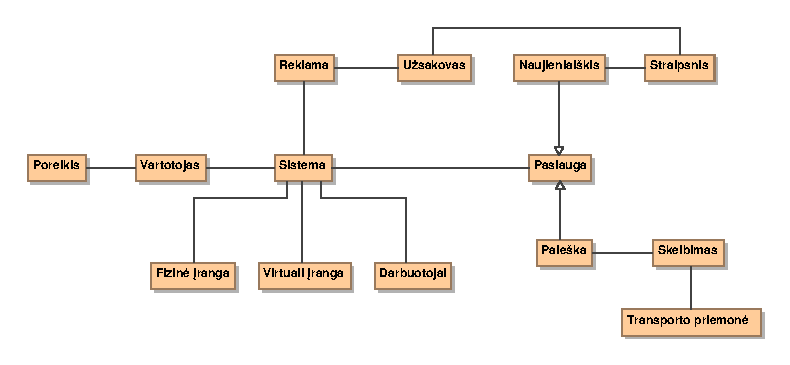
\includegraphics[width=\textwidth]{StatineSchema.eps}
			\caption{Dalykinės srities statinė struktūra\label{StaticStruct}}
		\end{center}
	\end{figure}

	Vartotojas naudojasi sistema siekdamas patenkinti savo poreikius. Sistema teikia šias paslaugas: naujienlaiškis, forumas, paieška. Paieškos rezultatas yra skelbimai su kiekvieno jų transporto priemonėmis. Užsakovas gali užsakyti reklamą arba straipsnį, kuris bus išplatintas sistemos naujienlaiškyje. Sistemą įtakoja jos fizinė ir virtuali įranga bei darbuotojai.
	\pagebreak
	
	\subsection{Užduotys}
	
	Žemiau esančiame \ref{UseCase3} paveikslėlyje vaizduojamos pagrindinės sistemoje atliekamos užduotys ir su jomis susiję agentai.
	
	\begin{figure}[h]
		\begin{center}
			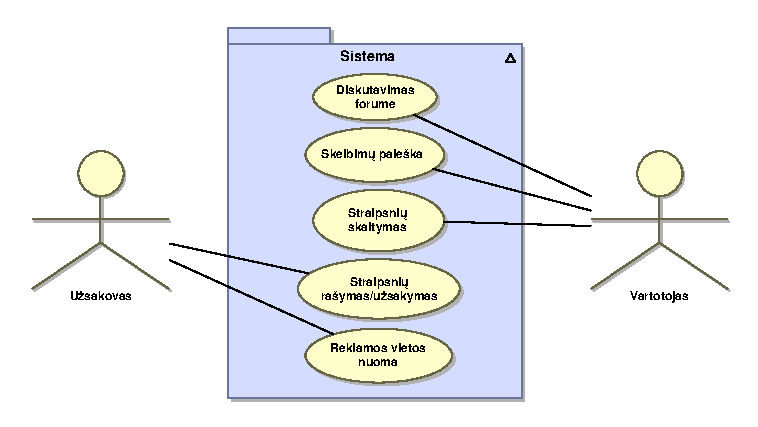
\includegraphics[width=\textwidth]{AnalUzduotys.eps}
			\caption{Užduotys\label{UseCase3}}
		\end{center}
	\end{figure}
	
	Vartotojas yra agentas, kuris naudodamasis sistemos teikiamomis paslaugomis dalyvauja forumo diskusijose, ieško skelbimų ir skaito straipsnius.
	
	Užsakovas yra agentas, kuris užsako reklamas ir rašo ar užsako straipsnius.
	\pagebreak
	
	\subsection{Užduočių vykdymo scenarijai}
	
	Žemiau pateikiamas užduoties „Skelbimų paieška“ vykdymo scenarijus:
	
	\begin{figure}[h]
		\begin{center}
			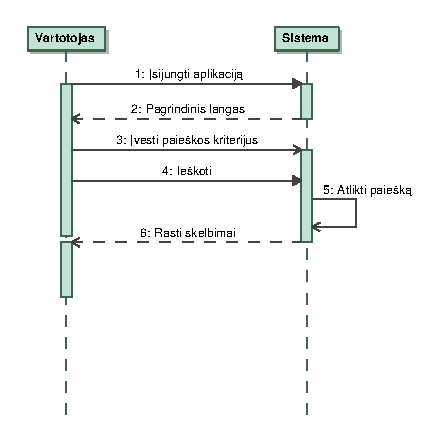
\includegraphics[width=0.8\textwidth]{PaieskaSeka.eps}
			\caption{Užduoties „Skelbimų paieška“ vykdymo scenarijus\label{SearchScenario}}
		\end{center}
	\end{figure}
	
	Vartotojas, įsijungęs aplikaciją, įveda paieškos kriterijus, pagal kuriuos nori ieškoti transporto priemonių skelbimų. Vartotojui patvirtinus pasirinkimą, sistema atlieka paiešką ir atvaizduoja visus kriterijus atitikusius skelbimus vartotojui aplikacijoje.
	\pagebreak
	
	Žemiau pateikiamas straipsnių skaitymo/rašymo užduočių vykdymo scenarijus:
	
	\begin{figure}[h]
		\begin{center}
			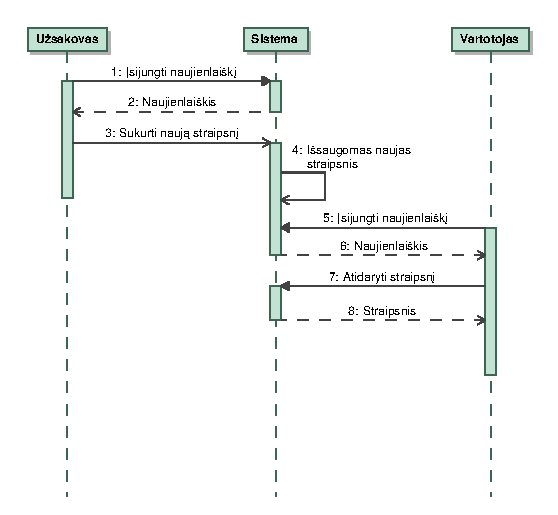
\includegraphics[width=0.8\textwidth]{Straipsniai.eps}
			\caption{Straipsnių skaitymo/rašymo užduočių vykdymo scenarijus\label{ArticleScenario}}
		\end{center}
	\end{figure}
	
	Užsakovas, įsijungęs naujienlaiškį, turi galimybę jame patalpinti naują straipsnį. Jam tai padarius, sistema straipsnį išsaugo ir jis dabar yra pasiekiamas visiems vartotojams. Vartotojas, atsidaręs naujienlaiškį, gali pamatyti šio straipsnio antraštę ir jį atidaryti.
	\pagebreak
	
	Žemiau pateikiamas užduoties „Diskutavimas forume“ vykdymo scenarijus:
	
	\begin{figure}[h]
		\begin{center}
			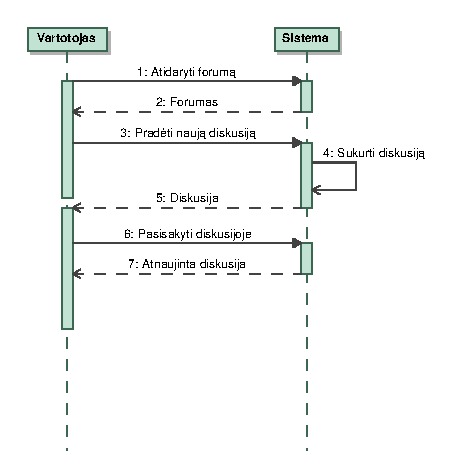
\includegraphics[width=0.8\textwidth]{Forumas.eps}
			\caption{Užduoties „Diskutavimas forume“ vykdymo scenarijus\label{ForumScenario}}
		\end{center}
	\end{figure}
	
	Vartotojas, įsijungęs forumą, gali sukurti naują diskusiją. Tada bet kuris vartotojas gali atsidaryti šią diskusiją ir patalpinti joje naują įrašą.
	\pagebreak
	
	\subsection{Dalykinės srities dinaminė struktūra}
	
	Žemiau pateikiamas esybės „Skelbimas“ gyyvavimo ciklas:
	
	\begin{figure}[h]
		\begin{center}
			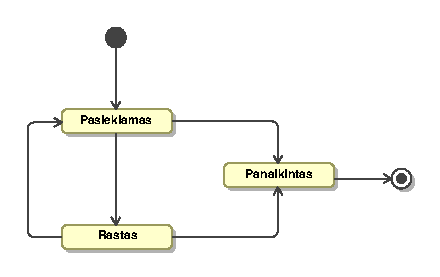
\includegraphics[width=0.8\textwidth]{SkelbimoBusena.eps}
			\caption{Esybės „Skelbimas“ gyyvavimo ciklas\label{AdvertState}}
		\end{center}
	\end{figure}
	
	Pradinė kiekvieno sistemos sekamo skelbimo būsena yra „Pasiekiamas“. Konkrečiam vartotojui vykdant skelbimų paiešką, skelbimas to vartotojo kontekste gali tapti „Atrastas“, jei jis atitiko vartotojo nurodytus paieškos kriterijus. Tam pačiam vartotojui pakartotinai atlikus paiešką, skelbimas gali vėl tapti „Pasiekiamas“, jei jis neatitiko vartotojo nurodytų kriterijų. Bet kokiu laiko momentu skelbimas gali tapti „Panaikintas“, jei jis bus ištrintas iš jo šaltinio, ir taip baigsis jo gyvavimo ciklas.
	\pagebreak	
	
	Žemiau pateikiamas esybės „Reklama“ gyyvavimo ciklas:
	
	\begin{figure}[h]
		\begin{center}
			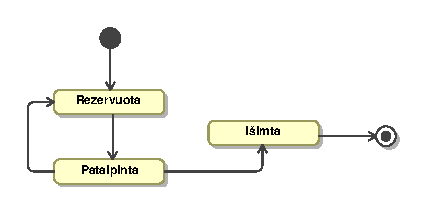
\includegraphics[width=0.8\textwidth]{ReklamosBusena.eps}
			\caption{Esybės „Reklama“ gyyvavimo ciklas\label{AdState}}
		\end{center}
	\end{figure}
	
	Pradinė užsakovo užsakytos reklamos būsena yra „Rezervuota“. Kai jai atsiranda laisva vieta ir yra galima ją rodyti, ji tampa „Patalpinta“. Pasibaigus reklamos rezervavimo laikui užsakovas gali ją pakartotinai užsakyti ir reklama vėl taps „Rezervuota“. Priešingu atveju ji bus „Išimta“ ir jos gyvavimo ciklas baigsis.
	\pagebreak	
	
	\section{Analizės rezultatai}
	
	Šiame skyriuje vidinė ir išorinė verslo proceso analizė apibendrinama pateikiant esmines įžvalgas SSGG (SWOT) lentelės (\ref{SWOT}) pavidalu.
	
	\begin{center}
		\captionof{table}{SSGG (SWOT)\label{SWOT}}		
		\begin{tabular}{ | c | c | }
			\hline
			\textbf{Stiprybės} & \textbf{Silpnybės} \\ \hline 
			\makecell{Unikalumas \\ Efektyvumas \\ Paprasta naudotis \\ Mažas darbuotojų skaičius \\ Paslaugos teikiamos 24/7} & \makecell{Priklausoma nuo kitų sistemų (šaltinių) \\ Uždirbama tik iš reklamų} \\ \hline
			\textbf{Galimybės} & \textbf{Grėsmės} \\ \hline
			\makecell{Įtraukti daugiau šaltinių \\ Didinti reklamai skirtą vietą \\} & \makecell{Šaltiniai nenori dalintis skelbimais \\ Balansas tarp turinio ir reklamos \\ Mažas vartotojų srautas} \\ \hline 
		\end{tabular}
	\end{center}
	\pagebreak	
	
	\section{Verslo proceso tobulinimo strategija}
	
	Verslas bus tobulinamas įdiegiant naujas, vartotojams naudingas, funkcijas, kurios padarytų naujos transporto priemonės ieškojimą dar patogesnį (pvz., būtų galima lyginti 2 ar 3 transporto priemones). Taip pat bus bandoma gerinti paieškos algoritmus (vartotojui rekomenduoti skelbimus, panašius į jo dažnai lankomus). Tai padės padaryti kiekvieną vartotojo praleistą minutę ieškant transporto priemonės daug prasmingesnę ir efektyvesnę, todėl tai sutaupytų vartotojui laiko.
	\bigskip	
	
	Siekiai:
	\begin{itemize}
		\item{Pagerinti ieškojimo sistemą:}
		\begin{itemize}
			\item{Rekomenduoti skelbimus atsižvelgiant į vartotojo veiklą,}
			\item{Vartotojui, pakartotinai naudojantis sistema, suteikti galimybę pratęsti paiešką nuo ten, kur baigė anksčiau.}
		\end{itemize}
		\item{Klientų informavimas:}
		\begin{itemize}
			\item{Pranešti vartotojui apie naują, galimai jį dominantį, skelbimą naudojant sistemą.}
		\end{itemize}
		\item{Padidinti funkcijų skaičių:}
		\begin{itemize}
			\item{Suteikti galimybę lyginti kelias transporto priemones.}
		\end{itemize}
	\end{itemize}
	\pagebreak
	
	\section{Sistemos naudojimo scenarijus}
	Šiame skyriuje aprašomas sistemos naudojimo pagrindinis scenarijus.
	
	\subsection{Scenarijus}
	Pagrindinis scenarijus, kai vartotojas naudojasi pagrindine paslauga (vykdo skelbimų paiešką), pavaizduotas \ref{Scenario} paveiklėlyje.
	
	\begin{figure}[h]
		\begin{center}
			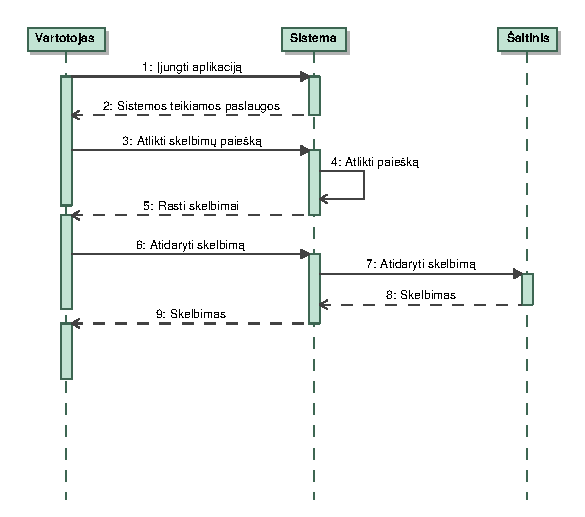
\includegraphics[width=0.8\textwidth]{Scenarijus.eps}
			\caption{Pagrindinis scenarijus\label{Scenario}}
		\end{center}
	\end{figure}
	
	\textbf{Įjungti aplikaciją} - vartotojas įsijungia aplikaciją, kuri teikia visas vartotojui prieinamas sistemos paslaugas.
	
	\textbf{Sistemos teikiamos paslaugos} - paslaugos, prieinamos vartotojui (skelbimų paieška, forumo diskusijos, naujienlaiškio straipsniai).
	
	\textbf{Atlikti skelbimų paiešką} - vartotojas pasirenka pagrindinę sistemos paslaugą (skelbimų paiešką).
	
	\textbf{Atlikti paiešką} - sistema pagal nustatytą algoritmą atrenka tik tuos skelbimus, kurie atitinka vartotojo nurodytus kriterijus.
	
	\textbf{Rasti skelbimai} - sistema vartotojui grąžina skelbimus, kurie patenkina jo nustatytus kriterijus.
	
	\textbf{Atidaryti skelbimą} - vartotojas, susidomėjęs skelbimu, gali jį  atidaryti. Tada sistema bando užmegzti ryšį su to skelbimo šaltiniu ir.
	
	\textbf{Skelbimas} - jei sistema užmezga ryšį su norimo skelbimo šaltiniu, ji nukreipia vartotoją į šaltinyje esantį (nebe šios sistemos) skelbimą.
	
	\subsection{Sistemos teikiama nauda}
	\ref{Gain} paveikslėlyje pavaizduota sistemos teikiama nauda.
	
	\begin{figure}[h]
		\begin{center}
			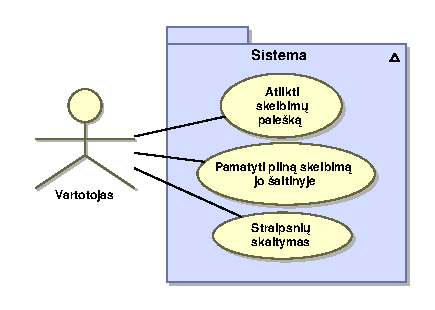
\includegraphics[width=0.9\textwidth]{Nauda.eps}
			\caption{Sistemos teikiama nauda\label{Gain}}
		\end{center}
	\end{figure}
	\pagebreak
	
	\subsection{Esama būklė}
	Esama infrastruktūra:
	\begin{enumerate}
		\item{Kompiuteris,}
		\item{Telefonas.}
	\end{enumerate}
	
	\subsection{Priemonės scenarijui įgyvendinti}
	Priemonės, reikalingos sistemai palaikyti:
	\begin{enumerate}
		\item{Serveris,}
		\item{Internetas,}
		\item{Duomenų bazė,}
		\item{Darbuotojai, prižiūrintys sistemą,}
		\item{Operacinė sistema,}
		\item{Programinė įranga.}
	\end{enumerate}
	\pagebreak
	
	\section{Įgyvendinamumo ir naudos analizė}
	
	Šiame skyriuje įvairiais aspektais nagrinėjamos galimybės įgyvendinti sistemą.
	
	\subsection{Operacinis įgyvendinamumas}
	
	\textbf{Inovaciniai slenksčiai:}
	\begin{itemize}
		\item{Kliento operacinė sistema gali būti per sena aplikacijai paleisti.}
		\item{Kientai gali nesinaudoti sistema, nes turinys yra preinamas atskirose svetainėse.}
	\end{itemize}
	
	\textbf{Inovacinių slenksčių panaikinimo būdai:}
	\begin{itemize}
		\item{Sukurti alternatyvą?}
		\item{Suteikti informacija apie sistemos patogumą, skelbimų paieškos palengvinimą.}
	\end{itemize}
	
	
	\subsection{Techninis įgyvendinamumas}
	Komanda gali įgyvendinti šią sistemą, nes domėjosi šia sritimi, yra pakankamai kvalifikuoti įgyvendinti sistemai.
	
	\pagebreak
	
	\subsection{Ekonominis įgyvendinamumas}
	
	\begin{itemize}
	\item{Fiksuotos išlaidos - 31 000 €:}
	\begin{itemize}
	\item{Sistemos sukūrimas – 30 000 € \href{http://howmuchtomakeanapp.com}{(iš čia)},}
	
	\item{Techninė įranga:}
	\begin{enumerate}
		\item{Kompiuteris - 700 €,}
		\item{Nepertraukiamo maitinmo šaltinis – 100 €,}
		\item{Periferiniai įrenginiai – 150 €,}
		\item{Tinklo įranga – 50 €.}
	\end{enumerate}
	\end{itemize}
	
	\item{Eksploatavimo išlaidos mėnesiui - 1 210 €:}
	\begin{enumerate}
		\item{Sistemos administratoriaus atlyginimas – 1 000 €,}
		\item{Internetas – 10 €,}
		\item{Serverio nuoma – 200 €.}
	\end{enumerate}
	
	\item{Sistemos nešamas pelnas:}
	\begin{itemize}
		\item{Visas pelnas būtų gautas iš aplikacijoje rodomų reklamų.}
		\item{Apsilankymų skaičius populiariausiame Lietuvoje automobilių skelbimų portale autoplius.lt – $\approx$ 300 000 per mėnesį \href{http://www.siteworthtraffic.com/report/autoplius.lt}{(iš čia)}.}
		\item{Vidutiniškai 2,1\% lankytojų paspaudžia ant reklamos.}
		\item{Iš vieno paspaudimo galima uždirbti $\approx$ 0,48 €.}
		\item{Jei kas mėnesį iš 300 000 lankytojų 6 300 paspaus ant reklamos, už kurią mokama 0,48 €, tikėtinas pelnas per mėnesį siektų 3 024 € ir sistema atsipirktų per 18 mėnesių.}
	\end{itemize}
	\end{itemize}
	
	\pagebreak
	\subsection{Juridinis įgyvendinamumas}
	Sistema nepažeis Lietuvos Respublikos asmens duomenų teisinės apsaugos įstatymo, nes bus saugomas tik kliento el. pašto adresas, kuriuo nebus dalinamasi su trečiaisiais asmenimis.
	\pagebreak
	
	\part*{Rezultatai}	
	\addcontentsline{toc}{part}{Rezultatai}
	Projektavimo dalyje pasitelkiant skirtingus sistemos pjūvius aprašyta knygų dalinimosi sistemos architektūra. Užduočių pjūvyje pasitelkiant užduočių ir sekų diagramomis išaiškinti pagrindiniai agentų (vartotojų ir administratorių) tikslai naudojantis sistema. Loginis pjūvis, pavaizduotas klasių ir objektų diagramomis, leido išskirti pagrindines esybes bei ryšius tarp jų. Kūrimo pjūvyje atlikta sistemos dekompozicija pradedant nuo bendro komponento toliau jį detalizuojant. Procesų pjūvyje, pasitelkiant veiklos diagramas, išskirti procesai, jų komunikacija, objektų gyvavimo ciklai. Galiausiai fiziniame pjūvyje apibrėžtas sistemos išdėstymas tinkle. Šis skirtingų požiūrių rinkinys leido aptikti ankčiau sukurtame sistemos prototipe buvusias klaidas bei išplėtoti tinkamą sistemos architektūrą.
	
	Reikalavimų dalyje yra atskleidžiami sistemos reikalavimai, kurie išskaidyti į funkcinius, nefunkcinius ir interfeiso reikalavimus. Funkciniuose reikalavimuose išvardijamos esminės sistemos funkcijos ir aprašomas vartotojo bei administratoriaus užduočių įgyvendinimas. Nefunkciniuose reikalavimuose yra apibrėžiamos neesminės sistemos funkcijos, įprasminančios pagrindines sistemos funkcijas. Interfeiso reikalavimai parodo, kaip sistemos atliekamos funkcijos turi būti pateiktos vartotojui, kad būtų patogu naudotis sistema.
	
	Dalykinės srities analizės dalyje pateiktas verslo proceso aprašas bei atlikta šio proceso išorinė analizė ir vidinė analizė, parodančios iš išorės atsirandančias galimybes ir grėsmes bei iš vidaus kylančias stiprybes ir silpnybes. Analizės rezultatai pateikti SSGG (SWOT) lentelės pavidalu. Pagal šiuos rezultatus sudaryta verslo proceso tobulinimo strategija. Galiausiai atlikta įgyvendinamumo ir naudos analizė, kurioje išsiaiškinta, ar ši sistema bus galima įgyvendinti ir ar ji teiks naudos.
	\pagebreak
	
	\part*{Išvados}	
	\addcontentsline{toc}{part}{Išvados}
	Remiantis projektavimo rezultatais bus galima sukurti mobiliesiems įrenginiams skirtą programėlę, kuri leis vienoje vietoje pasiekti automobilių skelbimus iš visos Europos, taip palengvindama paieškos procesą daugeliui žmonių.
	
	Reikalavimų dalis užtikrina, kad programuotojai vienareikšmiškai supras, kaip sistema turi atrodyti ir veikti ir tuo pačiu užtikrins, kad šia sistema bus galima lengvai pasinaudoti bet kokiam vartotojui.
	
	Dalykinės srities analizės metu buvo išsiaiškintos sistemos stiprybės, silpnybės, galimybės ir grėsmės bei būdai didinti sistemos stiprybes ir galimybes mažinant grėsmes ir silpnybes. Taip pat atlikta įgyvendinamumo analizė parodo, jog yra prasminga kurti šią sistemą.
	\pagebreak

	\part*{Terminų žodynas}
	\addcontentsline{toc}{part}{Terminų žodynas}	
	
	\bigskip
	\textbf{Vartotojas} - žmogus, besinaudojantis sistema.
	
	\textbf{Administratorius} - vartotojas, kuriam suteikiamos teisės tvarkyti šaltinius.
	
	\textbf{Skelbimas} - iš skelbimų šaltinio gautas sistemoje patalpintas skelbimas.
	
	\textbf{Šaltinis} - internetinis skelbimų puslapis, iš kurio gaunami skelbimai naudojami sistemoje.
	
	\textbf{Megstamas / mėgstamiausias} - skelbimas, kurį vartotojas išsaugo galimam lengvam ir greitam vėlesniam pasiekiamumui.
	\pagebreak

	\part*{Literatūros sąrašas}
	\addcontentsline{toc}{part}{Literatūros sąrašas}	
	
	Doug Rosenberg and Matt Stephens „Use Case Driven Object Modeling with UML“
\end{document}
